\section{State Estimation}
\label{sec:methods:state_estimation}

Adapting normalizing flow methods from parameter identification to state estimation introduces several non-trivial challenges. Unlike parameter identification, which targets a fixed set of unknown variables, state estimation requires the recovery of an entire sequential trajectory from partial observations. In Bayesian terms, the task is to approximate the posterior distribution $p(x_{1:T} | y_{1:T})$, which may be high-dimensional and multimodal. Standard filtering approaches, such as the Kalman filter, typically rely on known linear Gaussian dynamics. The setting considered here imposes no such restrictions: both the state dynamics and the observation model may be nonlinear and stochastic, and the resulting posterior can have a complex geometry. A naive strategy that applies a parameter identification method independently at each time step fails to model temporal dependencies between successive states and allows errors to accumulate over time.

Classical approaches address this problem with sequential Monte Carlo methods, such as particle filters \citep{Nemeth_2014}, which approximate the posterior by propagating a set of weighted particles through time. However, these methods are computationally expensive and suffer from degeneracy in high-dimensional state spaces. Variational approaches, including \acp{VAE} and RNN-based inference networks, have also been proposed for amortized state estimation (see Section~\ref{sec:literature:state_estimation}), but they often struggle to represent complex temporal dependencies and multimodal posteriors. 

To address these limitations, this section introduces four normalizing-flow-based methods for state estimation, ordered by increasing generality: Amortized State Flow, Latent State Space Model Flow (LatentSSMFlow), Normalizing Flow SDE (FlowSDE), and Conditional Stochastic Interpolant (CondStochInterpolant). For Amortized State Flow, we compare RealNVP and Flow Matching as the Bayesian inference backbones. For LatentSSMFlow, an exact invertible flow should be applied as the decoder, so RealNVP is implemented. For FlowSDE, the RealNVP architecture is used to model the diffusion term of a NeuralSDE. For CondStochInterpolant, the whole process can be seen as a refinement flow which transforms an observation-informed source distribution into the posterior state distribution.

All four methods are evaluated on the Lorenz-96 system \citep{lorenz1996predictability}, a canonical benchmark for nonlinear data assimilation. The state dimension is $N = 12$, and at each time step only $N/2 = 6$ components are observed, with additive Gaussian noise of varying magnitude. The governing equations are
\begin{equation}
    \frac{dx_i}{dt} = (x_{i+1} - x_{i-2})\,x_{i-1} - x_i + F, \qquad i = 1, \ldots, N,
    \label{eq:lorenz96}
\end{equation}
with periodic boundary conditions $x_{-1} = x_{N-1}$, $x_0 = x_N$, $x_{N+1} = x_1$, and forcing constant $F = 8$. This forcing regime produces sustained chaotic behavior.

\subsection{Amortized State Flow}
The most direct approach is to infer states across time by applying a normalizing flow independently to each observation segment. This reduces sequential state estimation to a collection of independent inference problems. Its main advantage is that the parameter-identification methods introduced in the preceding section can be transferred with minimal modification.
\begin{figure}[ht]
    \centering
    \includegraphics[width=0.7\textwidth]{figures/Amortized_state_flow.pdf}
    \caption{Architecture of amortized state estimation with normalizing flows.}
    \label{fig:amortized_state_flow}
\end{figure}
To introduce temporal structure into the latent variables, we use a Wiener process as the base distribution of the normalizing flow. This choice assigns monotonically increasing variance to successive latent variables while preserving a Gaussian distributional form, thereby providing an inductive bias toward smooth trajectories. The architecture is illustrated in Figure~\ref{fig:amortized_state_flow}.

This simplicity comes at a cost. Because each segment is processed as an independent set of observations, the method largely discards the temporal structure of the state trajectory. Long-range dependencies are not modeled, and estimation errors can propagate across segments without a corrective mechanism. Amortized State Flow is therefore most appropriate when the underlying dynamics are relatively smooth and only weakly dependent over time. It is less suitable when the dynamics are strongly nonlinear or when the observations are substantially noisy.

\paragraph{Numerical Results}
We first evaluate Amortized State Flow under different segment lengths on the partially observed Lorenz-96 system. The dataset contains $2000$ independent trajectories with horizon $H=100$, time step $dt=0.02$, and $500$ spin-up steps. Each initial state is sampled as a small Gaussian perturbation and then spun up before the training trajectory is recorded. The observation matrix selects every second state coordinate and the others remain unobserved. The observation noise is Gaussian with standard deviation $0.5$. The data are split into $1600$ training trajectories, $200$ validation trajectories, and $200$ test trajectories.

Since this method applies the flow independently to each observation segment, it is not expected to scale well to long windows. The purpose of this experiment is therefore to assess to what extent this simple amortized construction can still be used for state estimation as the segment length increases. Figure~\ref{fig:amortized_state_flow_segment_metrics} summarizes the quantitative performance, while Figure~\ref{fig:amortized_state_flow_segment_trajectories} shows representative reconstructed trajectories.

\begin{figure}[htbp]
    \centering
    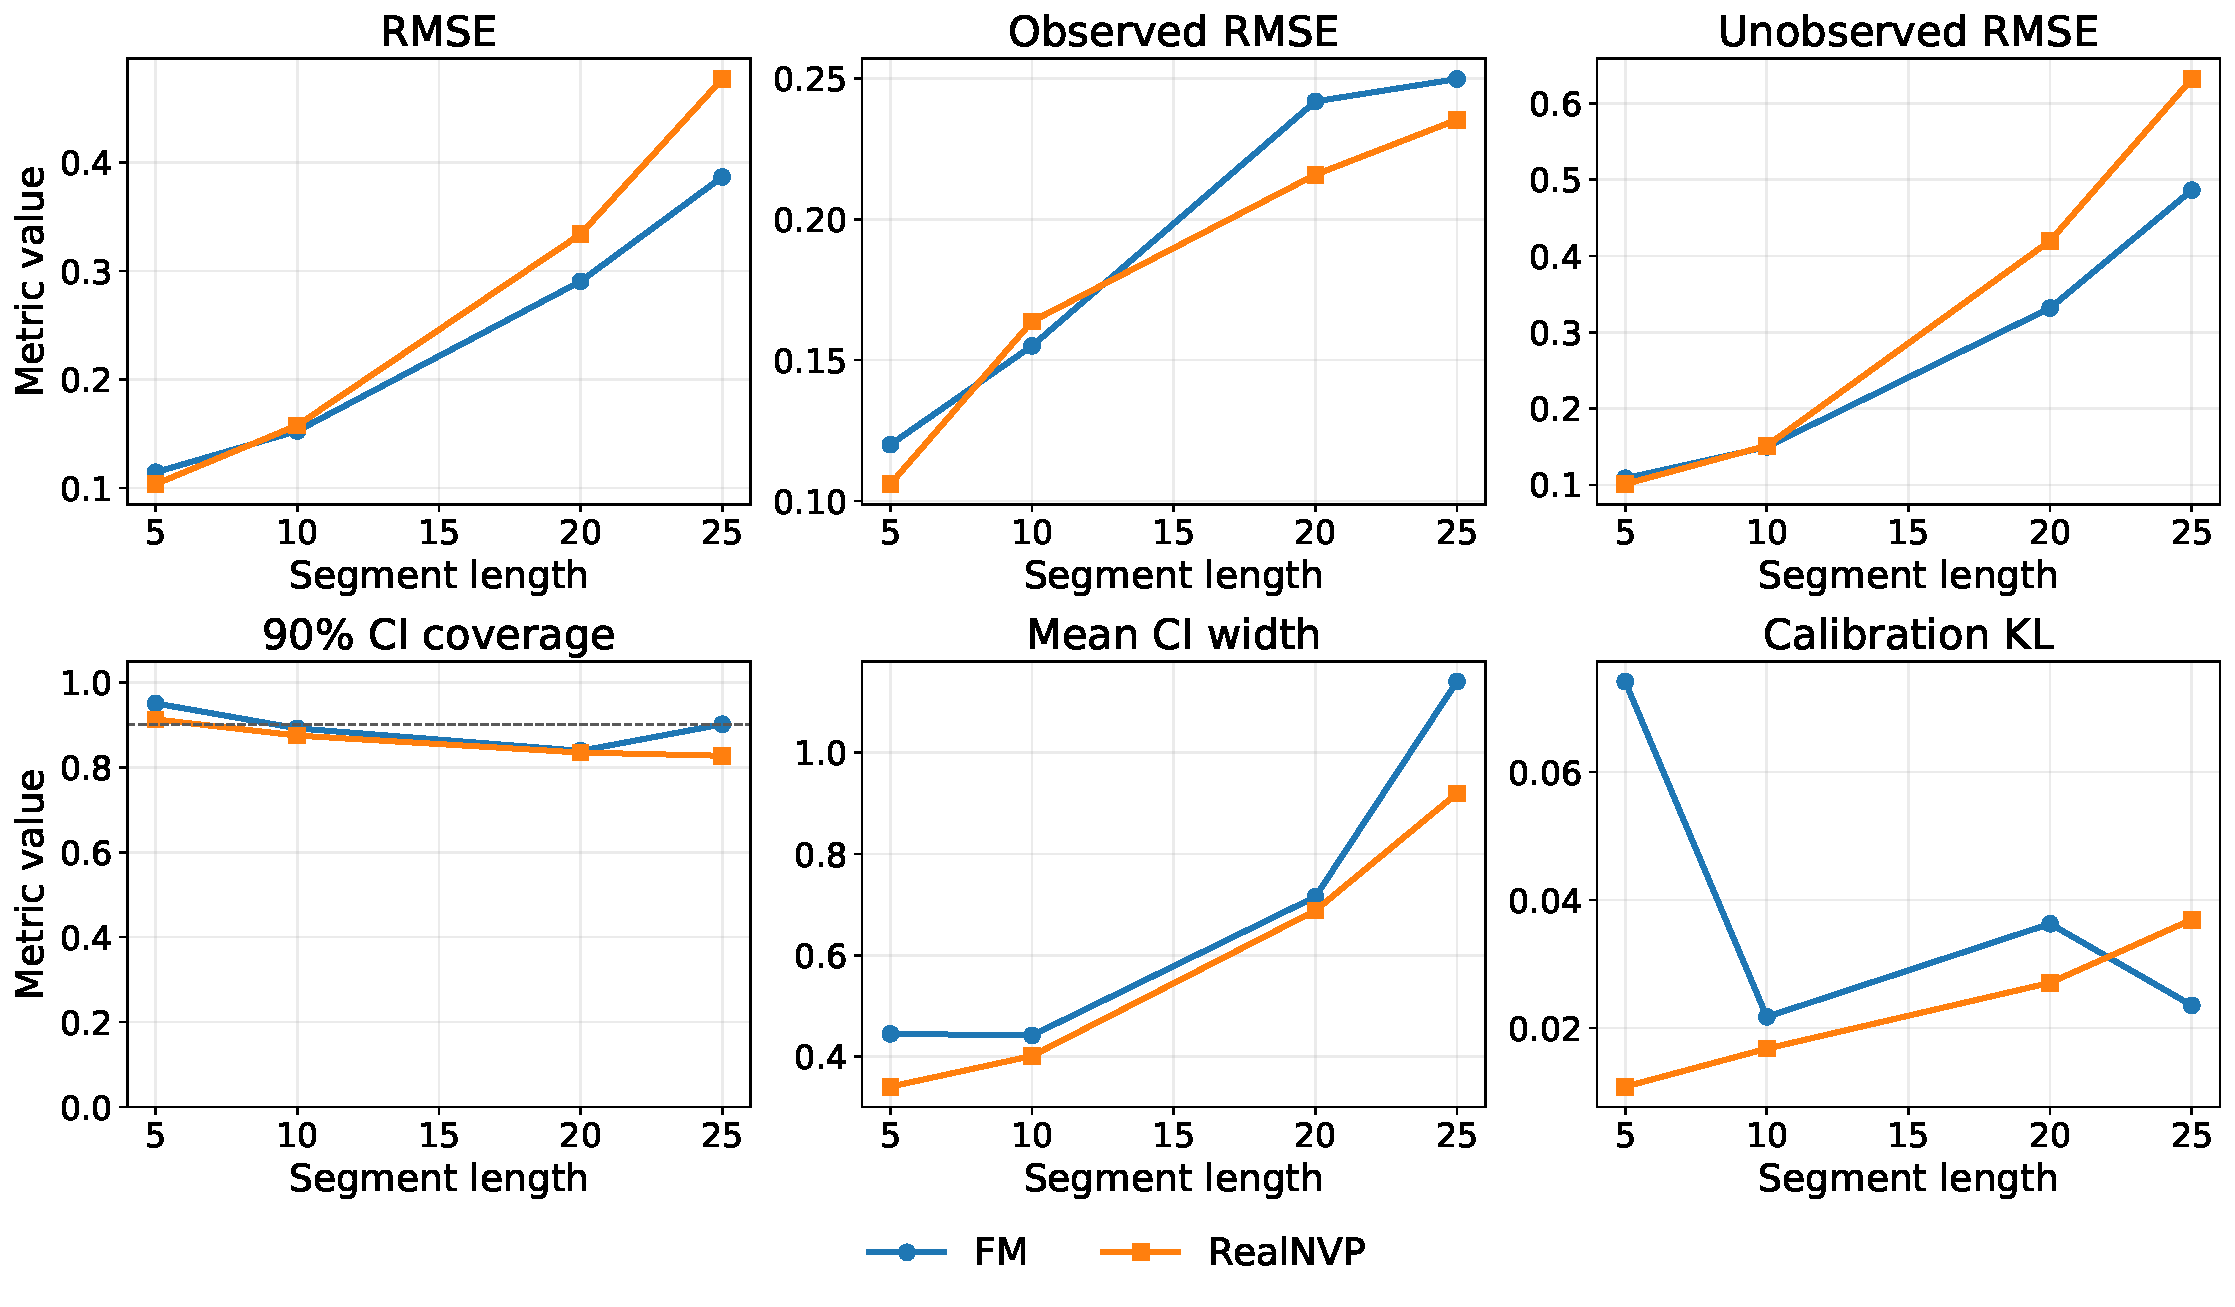
\includegraphics[width=\textwidth]{figures/amortized_state_flow_segment_comparison_metrics.pdf}
    \caption[Amortized State Flow Segment-Length Metrics]{Segment-length comparison for Amortized State Flow. The figure reports aggregate state-estimation metrics for different observation-window lengths, showing how the independent segment-wise inference strategy changes in accuracy and uncertainty calibration as more temporal context is provided to each segment.}
    \label{fig:amortized_state_flow_segment_metrics}
\end{figure}

\begin{figure}[htbp]
    \centering
    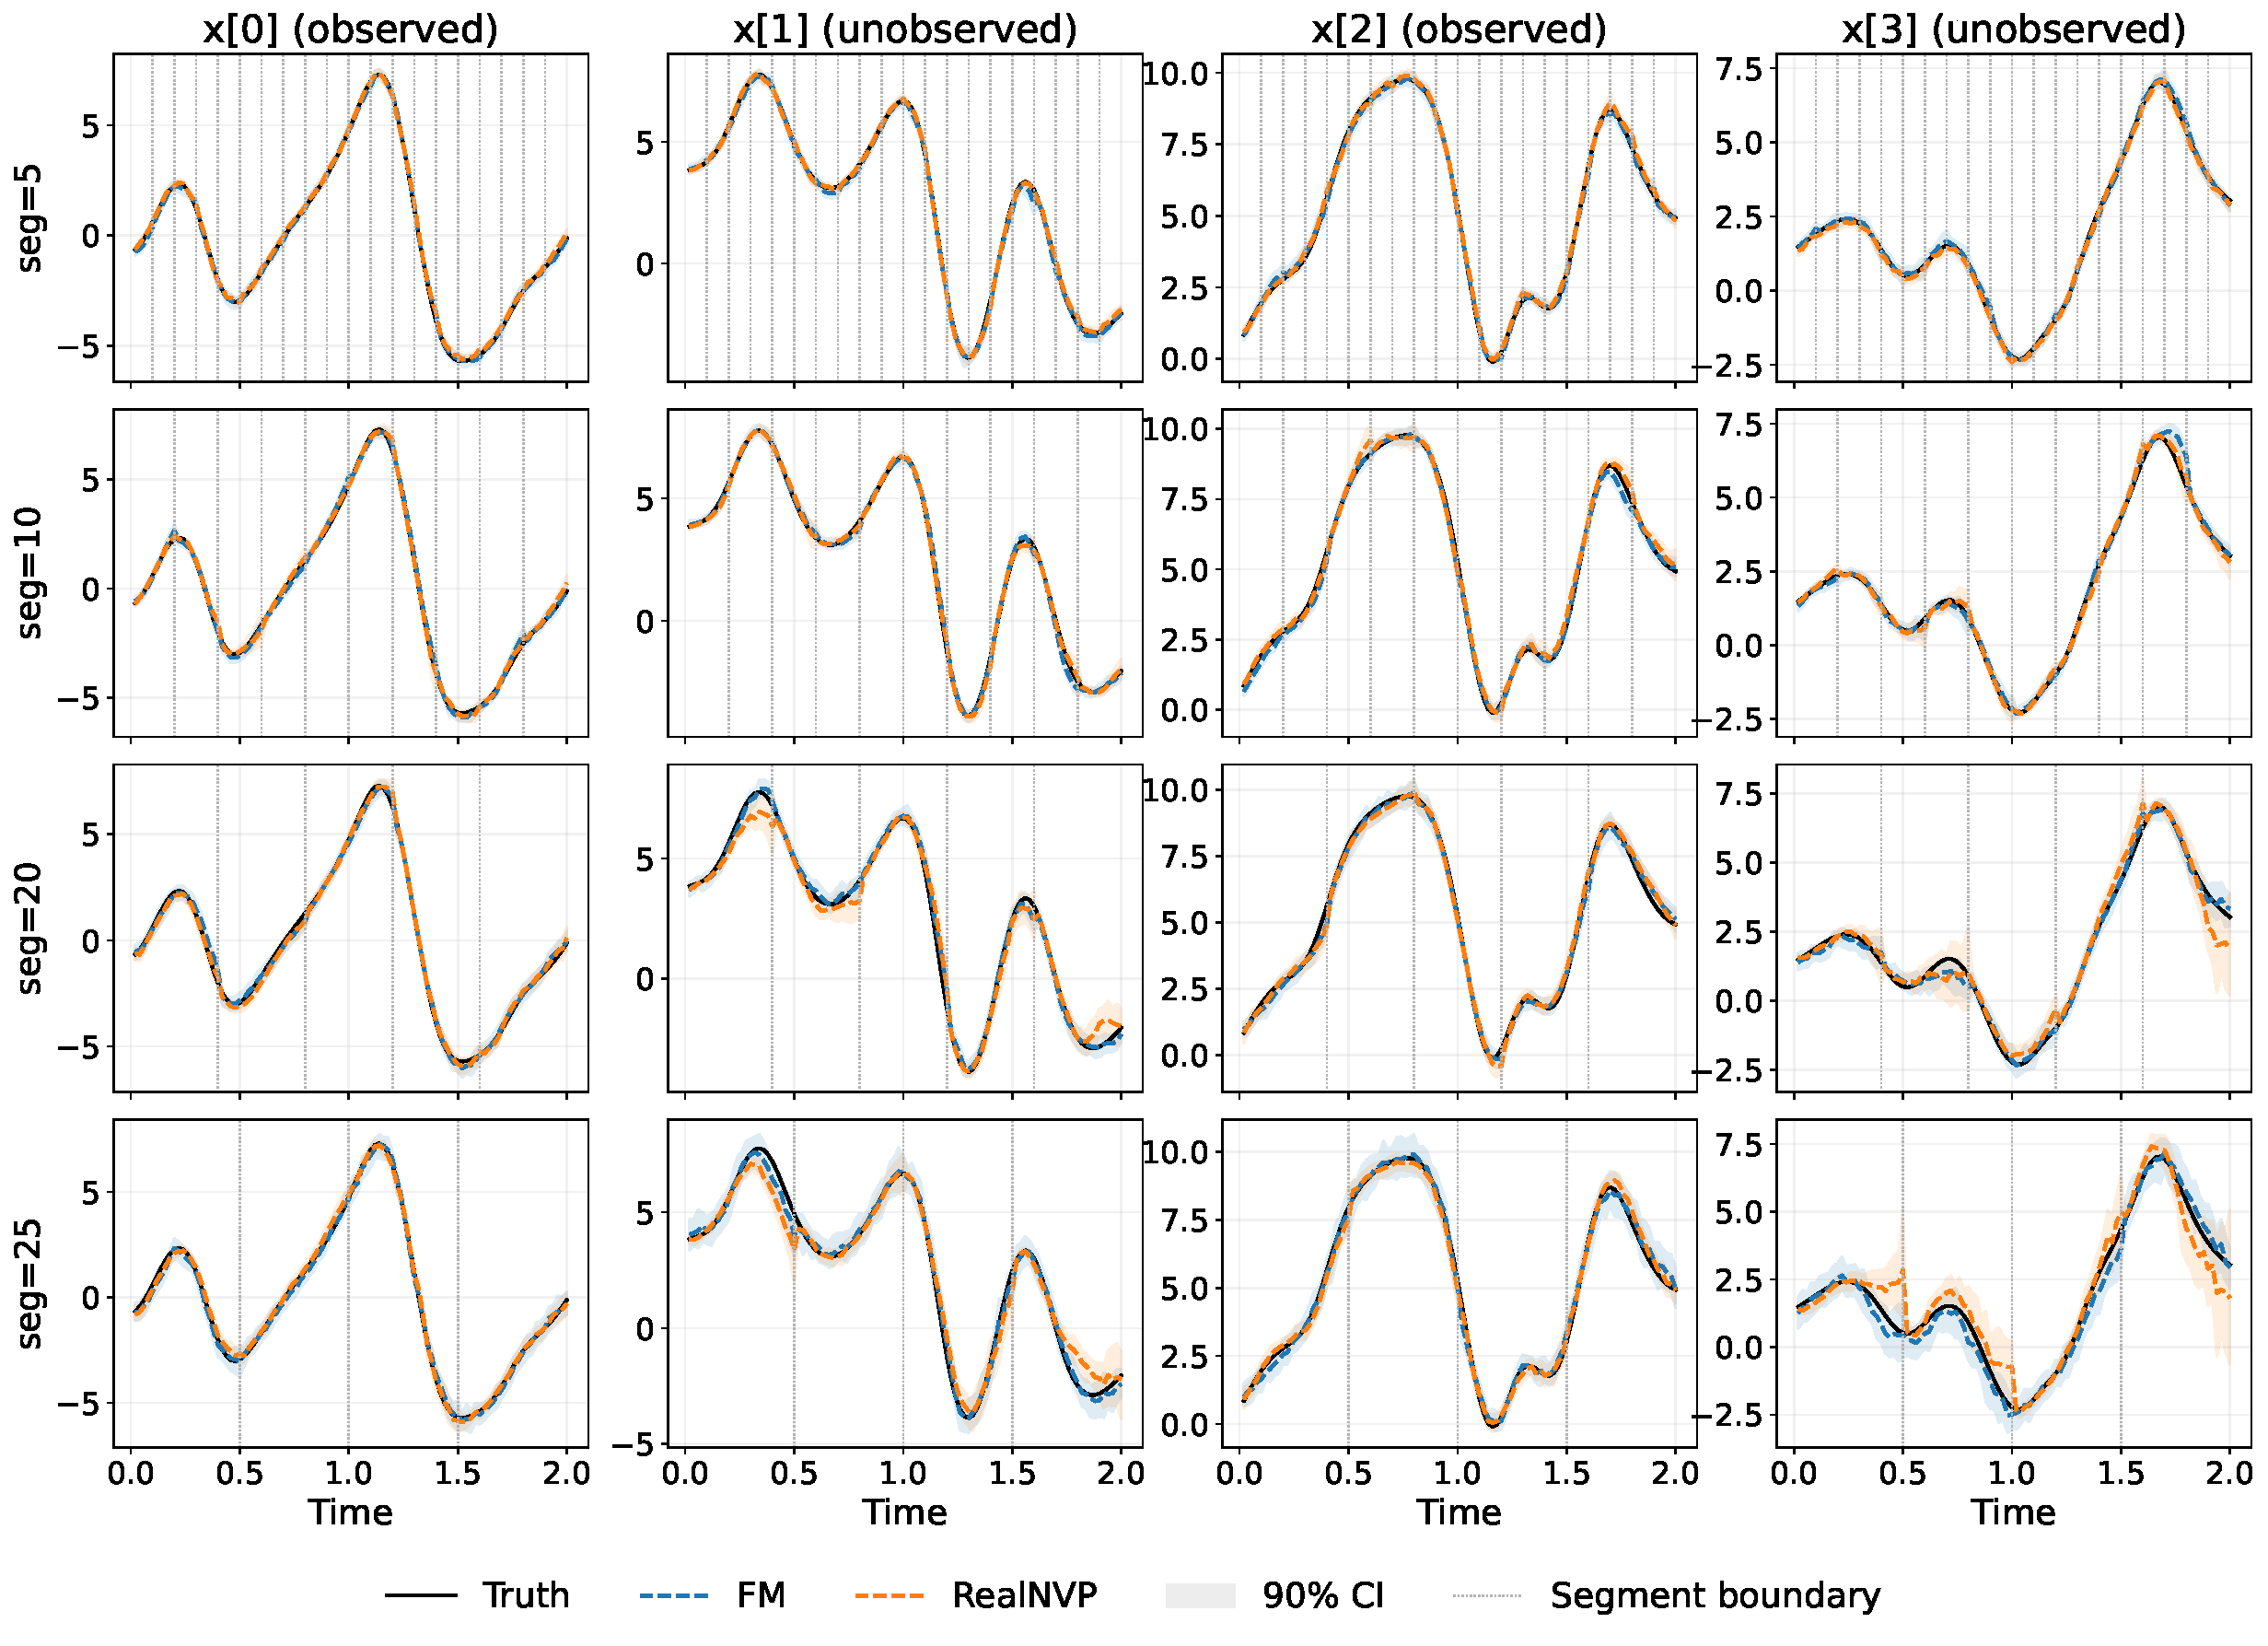
\includegraphics[width=\textwidth]{figures/amortized_state_flow_segment_comparison_trajectories.pdf}
    \caption[Amortized State Flow Segment-Length Trajectories]{Representative trajectory reconstructions obtained with Amortized State Flow for different segment lengths. The plots compare the estimated state trajectories with the reference dynamics and illustrate how segment-wise inference behaves across the physical time horizon.}
    \label{fig:amortized_state_flow_segment_trajectories}
\end{figure}

The comparison between RealNVP and Flow Matching highlights two different behaviors of the amortized estimator. RealNVP uses an explicitly invertible coupling architecture and is trained through likelihood maximization, which gives it a direct density-estimation objective for each segment. This often makes the posterior samples locally sharper and more stable when the observation window is short. Flow Matching, in contrast, learns a continuous transport vector field from the base process to the state trajectory distribution. Its estimates tend to vary more smoothly along the learned transport path, but the method is more sensitive to vector-field approximation and numerical integration errors. 

The quantitative results in Figure~\ref{fig:amortized_state_flow_segment_metrics} show that increasing the segment length decreases the amortized estimation precision. The total RMSE increases monotonically for both architectures. This degradation is mainly caused by the unobserved state components. Thus, the method can interpolate the directly observed coordinates reasonably well, but it becomes increasingly unreliable when reconstructing hidden coordinates over longer windows. Comparing the two architectures, RealNVP has a lower RMSE for the shortest segment length, but its error increases more rapidly than Flow Matching as the segment length grows. 

The uncertainty metrics lead to the same conclusion. The $90\%$ credible-interval coverage is close to the nominal level only for short windows; it drops below the nominal level at larger segment lengths. At the same time, the mean credible-interval width increases substantially, especially for Flow Matching. This indicates that the models respond to the harder long-window problem by broadening their posterior uncertainty, but the increased uncertainty is not sufficient to recover consistently calibrated intervals. The calibration KL comparison further suggests that RealNVP matches the uncertainty distribution of the observed components more closely than Flow Matching.

The trajectory reconstructions in Figure~\ref{fig:amortized_state_flow_segment_trajectories} explain this behavior visually. For segment lengths $5$ and $10$, both methods closely follow the reference trajectory for the shown state components, and the uncertainty bands remain narrow. At segment lengths $20$ and $25$, the estimates are still locally plausible, but deviations become visible around fast transitions and near segment boundaries. The effect is most evident in unobserved states $x[1]$ and $x[3]$, where the reconstructed trajectories begin to drift from the truth and the credible intervals widen. RealNVP shows sharper local estimates at short segment lengths, but its long-window reconstructions develop stronger boundary artifacts and larger errors in the unobserved components. Flow Matching is smoother and slightly more robust at the longest segment length, but it also requires wider uncertainty bands. Overall, these results show that Amortized State Flow is usable only for short local state-estimation windows; extending the segment length exposes the limitation of treating segments independently.

\subsection{Latent State Space Model Flow}
\label{sec:methods:latent_ssm_flow}
\begin{figure}[ht]
   \centering
   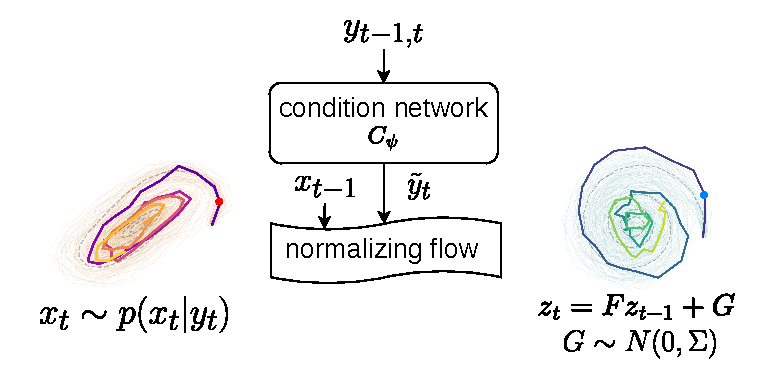
\includegraphics[width=0.7\textwidth]{figures/LinearSSMFlow.pdf}
   \caption{Architecture of Latent State Space Model Flow.}
   \label{fig:latent_ssm_flow}
\end{figure}

To overcome the limitation of treating time steps independently, we impose a linear Gaussian state-space model directly in the latent space of the normalizing flow. This yields the architecture termed LatentSSMFlow, shown in Figure~\ref{fig:latent_ssm_flow}. The model combines a structured temporal prior with a conditional normalizing flow decoder. Instead of using an independent standard Gaussian base distribution at each time step, the latent trajectory $z_{1:T}$ follows a Markovian Gaussian process:
\begin{equation}
z_t = F z_{t-1} + \eta_t, \qquad \eta_t \sim \mathcal{N}(0,\,Q).
\end{equation}
The transition matrix $F$ is fixed before training so that the latent dynamics remain contractive or non-expansive. This is enforced by bounding the spectral radius:
\begin{equation*}
    \rho(F) = \max_i |\lambda_i| \le \rho_{max} < 1,
\end{equation*}
where $\lambda_i$ denotes an eigenvalue of $F$. The process noise covariance is written as $Q=LL^\top$, where $L$ is a Cholesky factor. This parameterization guarantees that $Q$ is a valid positive semi-definite covariance matrix. Since the transition matrix $F$ is chosen to be stable, the latent linear Gaussian process has a stationary covariance $P_\infty$ satisfying the discrete Lyapunov equation $P_\infty = F P_\infty F^\top + Q$. We sample the initial latent state from $\mathcal{N}(0,P_\infty)$, so that the latent trajectory starts from the stationary distribution of the base process rather than from an arbitrary initial covariance.

The normalizing flow acts as a nonlinear decoder from the latent state space to the physical state space. At each step, it maps the latent variable $z_t$ to the state $x_t$, conditioned on an observation embedding $c_t$ and the previous state $x_{t-1}$. The conditioning vector $c_t$ is obtained from an encoder applied to the observations. In a filtering setting, this encoder may use only local information such as $y_t$ or $y_{t-1:t}$; in a smoothing setting, it may encode the full observation sequence $y_{1:T}$. Conditioning the flow on $x_{t-1}$ introduces an explicit first-order autoregressive dependence in the decoded state trajectory, while the latent \ac{SSM} provides a global temporal prior.

The likelihood formulation requires an exact invertible decoder. For RealNVP, each state can be transformed into latent space during training because the architecture is bijective:
\begin{equation}
    z_t = f_\phi^{-1}(x_t; c_t, x_{t-1}),\quad c_t=C_\psi(y_{t-1:t}).
\end{equation}
The model is then trained by \ac{MLE}. Using the change-of-variable formula, the log-likelihood of the state sequence is
\begin{equation}
    \log p(x_{1:T} | y_{1:T}) = \log p_{SSM}(z_{1:T}) + \sum_{t=1}^T \log \left| \det \frac{\partial f_\phi(x_t; c_t, x_{t-1})}{\partial x_t} \right|,
\end{equation}
where $p_{SSM}(z_{1:T})$ is the likelihood of the latent trajectory under the linear Gaussian state-space model. Thus, the latent dynamics are modeled by the state-space model, while the nonlinear state transition is learned by RealNVP.

Flow Matching, however, is not suitable for an equivalent LatentSSMFlow decoder. Because it has no exact inverse map and no tractable log-determinant, so the state trajectory cannot be mapped back to a latent trajectory whose probability is evaluated under $p_{SSM}(z_{1:T})$. Instead, the model is trained with a transport regression objective: samples from the latent \ac{SSM} prior are interpolated toward data states, and the network learns the corresponding velocity field. The latent \ac{SSM} therefore acts only as a source distribution for generation, not as a base measure coupled to the observed state trajectory through an exact change of variables. This distinction causes large training and evaluation mismatches. Thus, Flow Matching is omitted from the LatentSSMFlow comparison.

To improve training efficiency, we use a segmented multiple-shooting strategy. Each trajectory is divided into segments of length $T_s$. Within a segment, the model is unrolled autoregressively, so that prediction errors can influence later states in the same segment. Across segments, the initial state is anchored by the ground-truth state during training, and the segment computations can be parallelized. This strategy keeps the temporal training problem tractable while still exposing the model to multi-step state evolution.

\paragraph{Numerical Results}
We evaluate the RealNVP-based LatentSSMFlow with the same Lorenz-96 dynamics, observation mask, trajectory length, and train-validation-test split as in the previous experiment. The main difference is the observation-noise model. To challenge the uncertainty modeling ability of LatentSSMFlow, the observation noise follows a Student-$t$ distribution with $\nu=5$ degrees of freedom and scale $0.5$. Equivalently, the noise can be written as the Gaussian scale mixture
\begin{equation}
    \tau \sim \mathrm{Gamma}(\nu/2,\nu/2),\qquad
    e \sim \mathcal{N}(0,I),\qquad
    \eta_t = 0.5\,\frac{e}{\sqrt{\tau}}.
\end{equation}
The marginal noise variance is therefore $\nu(\nu-2)^{-1}0.5^2=5/12\approx0.4167$, corresponding to a marginal standard deviation of approximately $0.646$. This heavier-tailed observation model makes the evaluation more challenging by allowing occasional large observation errors, similar to outlier-contaminated measurements in real systems.

During training, the previous state provided to the decoder is the ground-truth state and the training is based on segmented trajectories. In the results shown here, we use the model trained with segment length $T_s=25$. Evaluation is then performed as a continuous autoregressive rollout over the full horizon. At the beginning of a test trajectory, the model is initialized from the given initial state. Thereafter, the previous state provided to the decoder is the model's own previous inferred state. Thus, the rollout tests whether LatentSSMFlow can maintain a coherent state estimate when its predictions are recursively fed back into the model. Although the model is trained on shorter multiple-shooting segments, the evaluation itself is carried out over the full $100$-step horizon.

Figure~\ref{fig:latent_ssm_flow_rollout_trajectories} shows representative full-horizon rollout trajectories, while Figure~\ref{fig:latent_ssm_flow_rollout_uncertainty_distribution} compares the learned posterior uncertainty with the observation-noise distribution.

\begin{figure}[htbp]
    \centering
    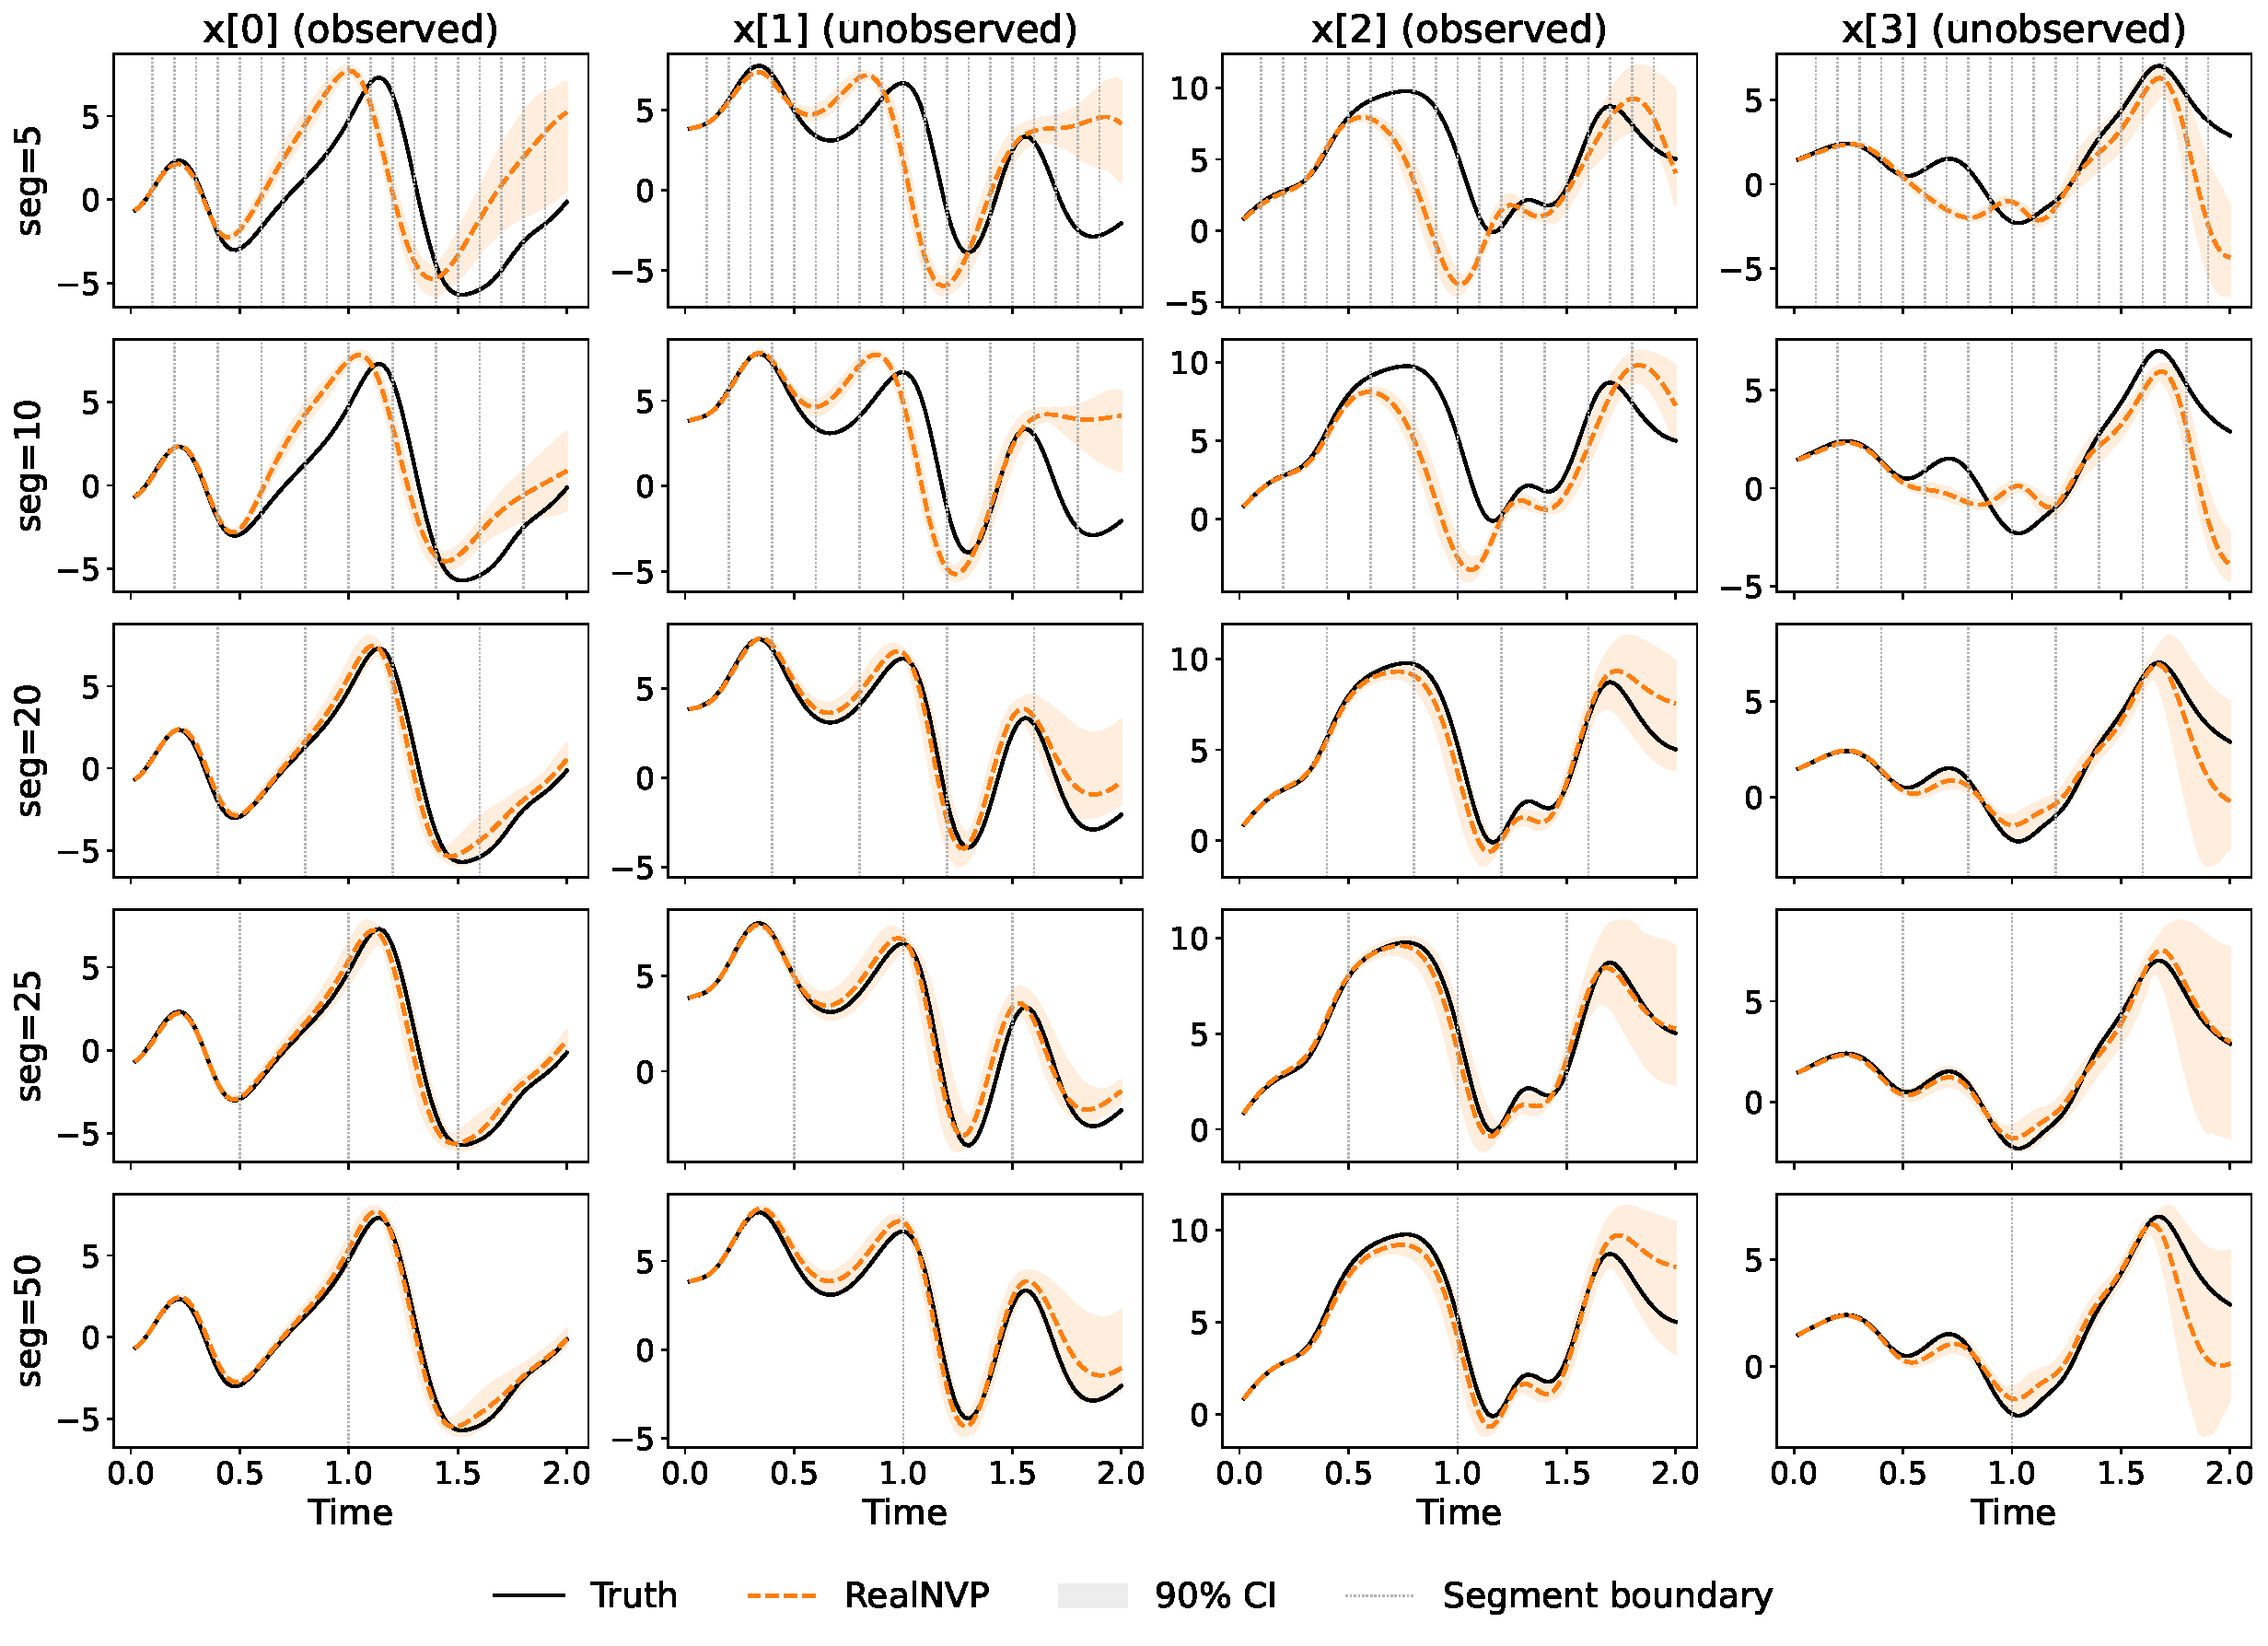
\includegraphics[width=\textwidth]{figures/latent_ssm_flow_100horizon_rollout_comparison_trajectories.pdf}
    \caption[LatentSSMFlow Full-Horizon Rollout Trajectories]{Full-horizon rollout trajectories obtained with the RealNVP-based LatentSSMFlow trained with segment length $T_s=25$. The plots show observed and unobserved components over the full $100$-step horizon.}
    \label{fig:latent_ssm_flow_rollout_trajectories}
\end{figure}

\begin{figure}[htbp]
    \centering
    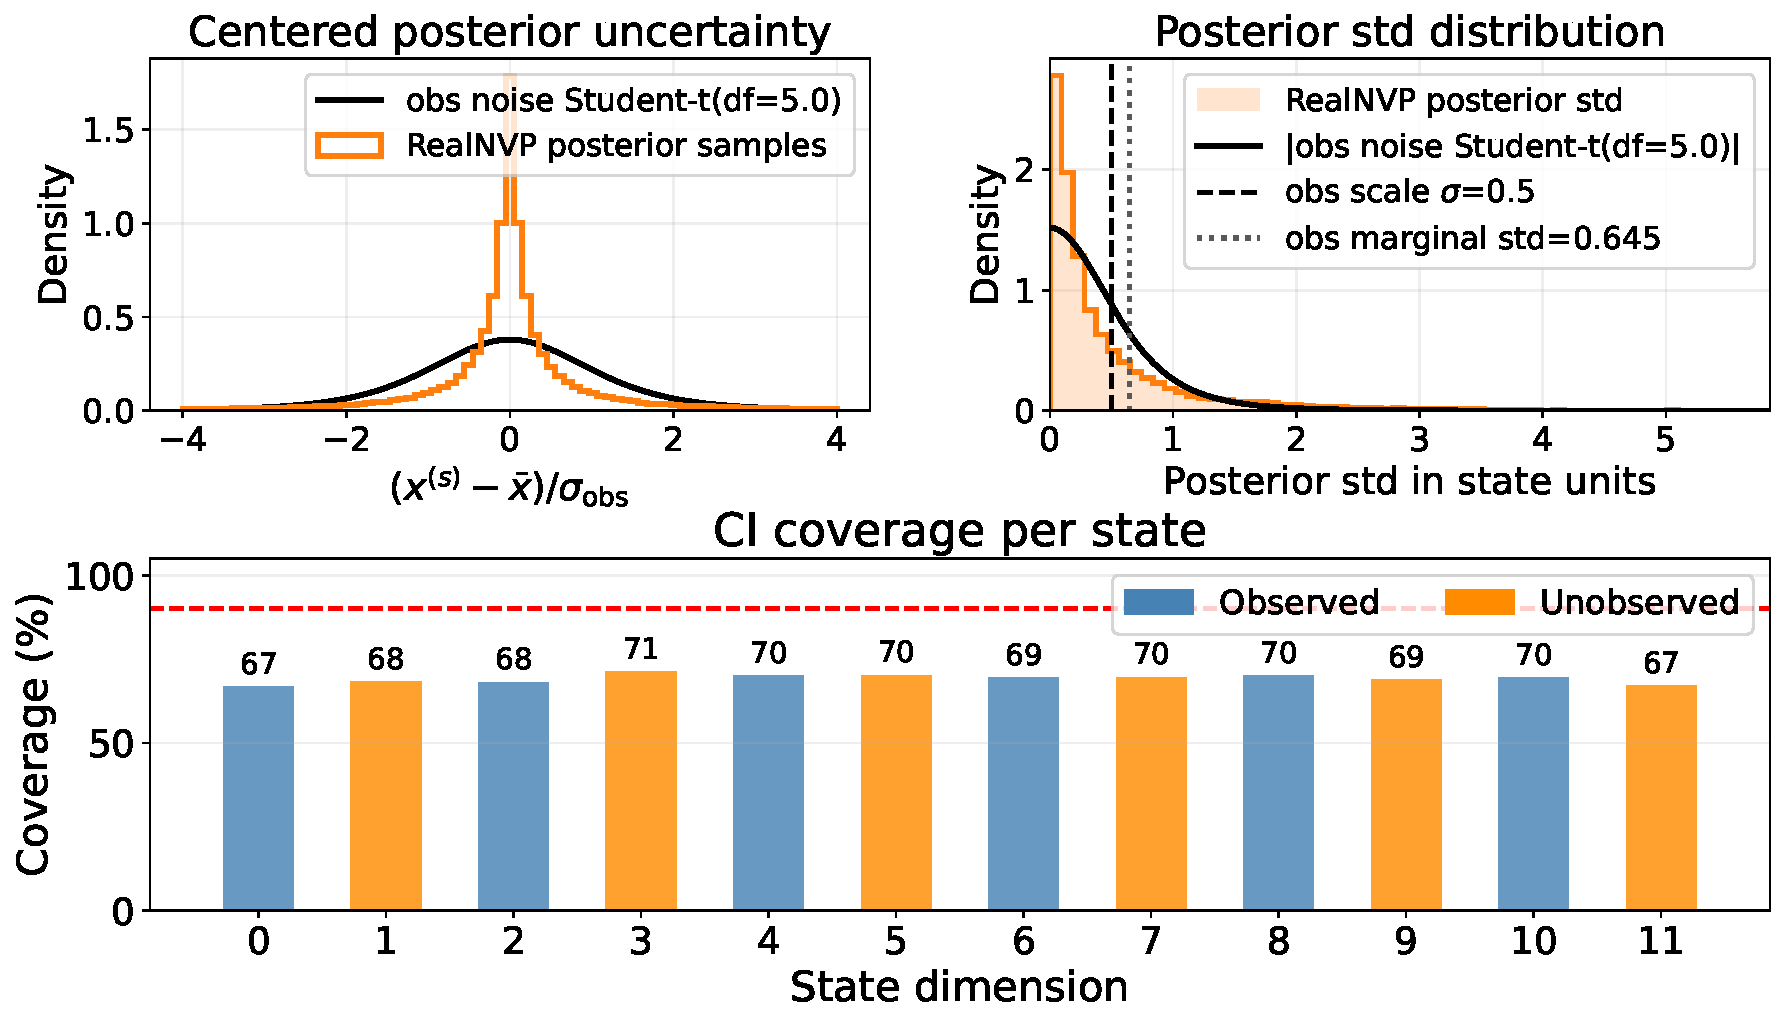
\includegraphics[width=0.8\textwidth]{figures/latent_ssm_flow_100horizon_rollout_comparison_uncertainty_distribution.pdf}
    \caption[LatentSSMFlow Full-Horizon Uncertainty Distribution]{Uncertainty analysis for the RealNVP-based LatentSSMFlow trained with segment length $T_s=25$ during full-horizon rollout. The left panel compares centered posterior samples with the Student-$t$ observation-noise distribution after normalization by the observation scale. The middle panel compares the posterior standard-deviation distribution with the observation scale and marginal observation-noise standard deviation. The right panel reports the empirical $90\%$ credible-interval coverage for each state dimension.}
    \label{fig:latent_ssm_flow_rollout_uncertainty_distribution}
\end{figure}

Figure~\ref{fig:latent_ssm_flow_rollout_trajectories} demonstrates the main advantage of LatentSSMFlow over the purely amortized segment-wise estimator. With $T_s=25$, the rollout closely follows the reference trajectory for both observed and unobserved components over the full horizon. Since the previous state during evaluation is the model's own inferred state, this result shows that the learned latent \ac{SSM} prior and autoregressive decoder can propagate state information through time. The method therefore supports continuous state estimation rather than only local segment reconstruction.

The full-horizon rollout also clarifies the role of the latent state-space structure. Although the model is trained on segmented trajectories, the inferred state can be propagated beyond the training segment length because the decoder is conditioned autoregressively on the previous estimate and the latent prior imposes temporal structure. This behavior contrasts with Amortized State Flow, where increasing the observation window does not introduce explicit coupling between adjacent estimates. In LatentSSMFlow, the autoregressive dependence on the inferred previous state allows information to be carried forward across the entire horizon.

The main limitation remains uncertainty modeling. Figure~\ref{fig:latent_ssm_flow_rollout_uncertainty_distribution} shows that the centered posterior samples are more concentrated around zero than the Student-$t$ observation-noise distribution, whose heavier tails represent occasional large observation errors. The posterior standard-deviation distribution also places a large amount of mass below the observation scale $0.5$ and the marginal Student-$t$ noise standard deviation, although it has a long right tail for some samples. This indicates that the model can express varying uncertainty across time and states, but its typical posterior spread is still too narrow.

The per-state coverage panel confirms this under-dispersion. The empirical coverage of the nominal $90\%$ credible intervals is only about $70\%$ across the twelve state dimensions, and both observed and unobserved coordinates show similar undercoverage. Thus, the calibration problem is not restricted to the hidden states; it is a global feature of the posterior. Overall, LatentSSMFlow improves continuous state reconstruction by introducing latent temporal dynamics and autoregressive feedback, but the RealNVP posterior remains overconfident under heavy-tailed observation noise.

\subsection{Normalizing Flow SDE}
To further increase the capacity for modeling dynamics and stochasticity, we estimate the state trajectory by representing the underlying dynamics as a stochastic differential equation. We define the conditional state $x_t| y_t$ as the new system variable $z_t$. When the state evolves continuously in time, its dynamics can be written as
\begin{equation}
    dz_t = f(z_t, t)\; dt + g(z_t, t)\;{\color{Orchid} dW_t},\quad dW_t={\color{Orchid} \sqrt{dt}\;\epsilon}, \quad \epsilon\sim \mathcal{N}(0, I).
\end{equation}
By modeling $f$ and $g$ with neural networks, the model can represent nonlinear dynamics and state-dependent noise. However, training a NeuralSDE by directly maximizing the likelihood of the observed data can cause the stochastic component to collapse, since the networks may learn to ignore the diffusion term and fit the dynamics mainly through the drift.

One way to improve the expressiveness of the diffusion term is to use variational inference, as in LatentSDE \citep{li2020scalablegradientsstochasticdifferential}. LatentSDE defines both a prior NeuralSDE and a posterior NeuralSDE, sharing the same diffusion function but using different drift functions. Because the diffusion term is shared, the KL divergence between the two stochastic processes is analytically tractable, allowing the model to be trained by maximizing the \ac{ELBO}. Another approach treats a NeuralSDE as an infinite-dimensional \ac{GAN} \citep{kidger2021neuralsdesinfinitedimensionalgans}. In this framework, the NeuralSDE acts as a generator that transforms Brownian motion into sample paths, while a Neural Controlled Differential Equation (NeuralCDE) acts as a discriminator on continuous-time trajectories. By optimizing a Wasserstein-type objective, this method can match the full distribution of generated paths to the data distribution in path space.

\subsubsection{Integration of Normalizing Flow in NeuralSDE}
Both approaches, however, require substantial computational resources and careful tuning. To reduce this burden, we incorporate a normalizing flow directly into the NeuralSDE framework, avoiding the need for an additional differential equation to support training. For computational efficiency, we use the RealNVP architecture to model the diffusion term. Taking a standard normal random variable $\epsilon\sim \mathcal{N}(0, I)$ as the latent variable of the flow gives the following modified SDE:
\begin{equation}\label{eq:flow_sde}
    dz_t = f_\theta(z_t, t)\; dt + g_\phi({\color{Orchid} \epsilon}; z_t, t) \; {\color{Orchid}\sqrt{dt}}, \quad \epsilon\sim \mathcal{N}(0, I),
\end{equation}
where $f_\theta$ is the drift function and $g_\phi$ is the normalizing flow. 

The factor $\sqrt{dt}$ is included so that the flow-generated random increment has the same time scaling as a standard \ac{SDE} diffusion term, where the variance of the stochastic step scales linearly with time ($\mathcal{O}(dt)$). Decoupling the normalizing flow's input from the time step $dt$ avoids this noise collapse and preserves a genuine continuous-time diffusion process.

Unlike standard amortized Bayesian inference, the normalizing flow is not trained by minimizing a KL divergence against an available ground-truth posterior. Instead, the flow is used only in the forward stochastic direction and the latent variable $\epsilon$ is sampled from its standard normal distribution during training. Then, FlowSDE is trained by maximizing the likelihood of the observed data, which requires integrating the SDE (Equation~\ref{eq:flow_sde}) through time. Several SDE solvers can be chosen, such as Euler--Maruyama, Heun, Midpoint, Milstein, or reversible Heun. The initial state is supplied to FlowSDE as part of the initial value problem and is then evolved by the SDE over all state coordinates; it is not inferred by a separate network.

The flow captures complex dependencies between the stochastic input and the current state, enabling the model to learn richer stochastic dynamics. An advantage of RealNVP is its simple Jacobian determinant, which simplifies likelihood computation and supports efficient training. However, unlike NICE, RealNVP is non-volume-preserving. In order to prevent variance collapsing, we apply a hyperbolic tangent ($\tanh$) clamping to the raw neural network scale output, parameterizing each diagonal scale factor as $\exp(\alpha \cdot \tanh(\cdot))$, where $\alpha > 0$ is a bounding hyperparameter. This restricts the scale factors to the open interval $(e^{-\alpha}, e^{\alpha})$. Thus, the RealNVP preserves the capacity to represent expressive, varying noise levels across the state space without suffering from stochastic collapse or gradient explosion.

\subsubsection{Training FlowSDE}
The training objective is formulated probabilistically to prevent noise collapse. Rather than minimizing a deterministic trajectory-matching loss (such as \ac{MSE}), which can force the diffusion term to zero, we minimize the \ac{NLL}. It combines the likelihood of the full state trajectory estimated by the SDE with the continuous-time transition likelihood (the normalizing flow loss) of the latent trajectory. Specifically, assuming a Gaussian state likelihood, the state loss is:
\begin{equation}
    \mathcal{L}_{\text{state}}
    =
    \sum_{t} -\log \mathcal{N}\left(x_t; z_t, \sigma_{\text{state}}^2 I\right),
\end{equation}
where $x_t$ is the reference full state and $\sigma_{\text{state}}^2$ controls the assumed state-likelihood variance.

To compute the transition loss $\mathcal{L}_{\text{trans}} = \sum_{t} -\log p(z_{t+dt} | z_t)$ under discretization in Equation~\ref{eq:flow_sde}, we apply the change-of-variables formula of normalizing flows:
\begin{equation}
    \mathcal{L}_{\text{trans}} = \sum_{t} \left( \frac{1}{2} \|\epsilon\|^2 + \log \left| \det \frac{\partial g_{\phi}(\epsilon; z_t, t)}{\partial \epsilon} \right| + \frac{D}{2}\log(2\pi dt) \right),
\end{equation}
where $D$ is the dimension of the state space. The standard Gaussian negative log-likelihood of the latent variable $\epsilon$ is a constant. So the transition loss simplifies to the term of Jacobian determinant. It is worth to note that there is a term related to $dt$ in the transition loss, which reflects the time scaling of the diffusion term. For a fixed-step solver, this term is constant and does not affect the optimization. For an adaptive-step solver, since the solver internal step does not directly affect the network parameters, the gradient of this term is still zero. Unless exact probability density is required, an actual $dt$ used by the solver is not needed. Therefore, the $dt$-term can be treated as a constant during training.

Compared with the previous two methods, FlowSDE is more general: it can represent nonlinear long-term dynamics and state-dependent noise. This expressiveness comes with higher computational cost and more challenging training, since the \ac{SDE} must be integrated while the neural networks are optimized.

We apply a multiple shooting framework to stabilize training and mitigate the exploding or vanishing gradients common in chaotic systems. The full trajectory horizon $T$ is divided into $K$ shorter segments of length $T//K$. On each segment $k \in \{1, \dots, K\}$, the SDE is integrated independently starting from a supplied segment-specific initial state $z_0^{(k)}$. To address chaotic sensitivity, partial observability, and trajectory disjointedness, three strategies are integrated into this framework:
\begin{itemize}
    \item \textbf{Continuity Constraints:} To force the disjointed segments to form a single continuous trajectory in the continuous-time limit, we add a consistency penalty to the overall training loss:
    \begin{equation}
        \mathcal{L}_{\text{cont}} = \sum_{k=1}^{K-1} \| z_{\text{end}}^{(k)} - z_0^{(k+1)} \|^2
    \end{equation}
    where $z_{\text{end}}^{(k)}$ is the terminal state predicted at the end of the $k$-th segment.
    \item \textbf{Given Initial States:} The initial state $z_0^{(k)}$ of each segment is provided directly to the SDE solver. No amortized inference network or reparameterized initial-state distribution is used. Consequently, uncertainty in the initial state is not modeled by FlowSDE; the learned stochasticity describes the subsequent state evolution conditioned on the supplied initial state.
    \item \textbf{Curriculum Learning:} To prevent chaotic divergence during early training epochs, we implement a curriculum on the segment length. We begin training with highly localized horizons (e.g., $T//K = 5$ steps) and incrementally increase $T//K$ to the full multiple shooting length as the drift and diffusion dynamics converge.
\end{itemize}

\begin{figure}
    \centering
    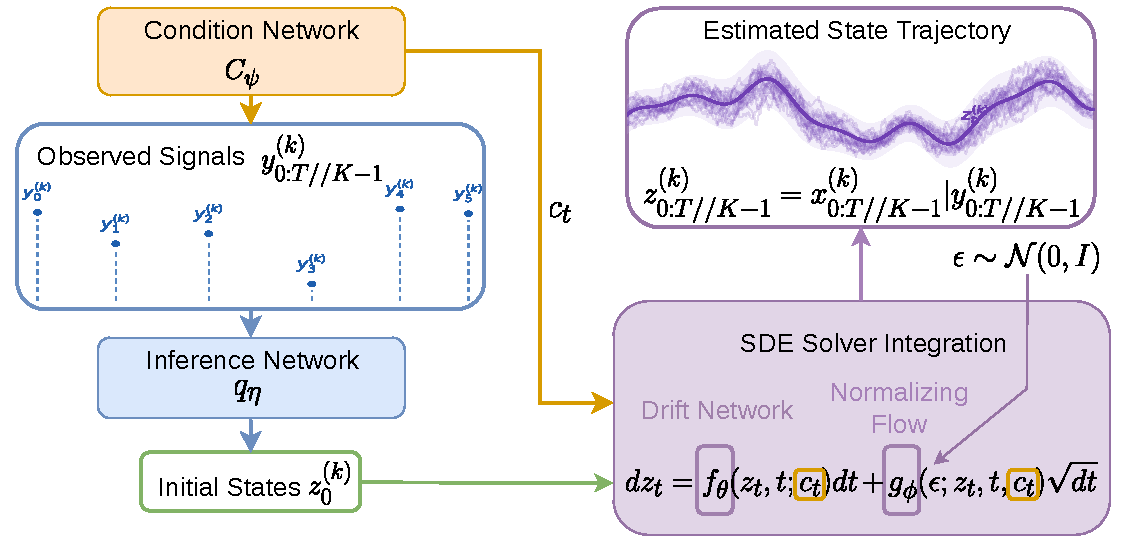
\includegraphics[width=0.9\textwidth]{figures/FlowSDE.pdf}
    \caption[Computational graph of FlowSDE]{Computational graph of FlowSDE. For the $k$-th segment of length $T//K$, the supplied initial state $z_0^{(k)}$ initializes the SDE solver directly. The drift network $f_\theta$ and diffusion network $g_\phi$ model the deterministic and stochastic dynamics, respectively. The condition $c_t$ is extracted from the segment observations by the condition network $C_\psi$. The stochastic solver integrates all state coordinates forward in time using FlowSDE.}
    \label{fig:flow_sde_graph}
\end{figure}
To sum up, the overall computational graph for FlowSDE is illustrated in Figure~\ref{fig:flow_sde_graph}.

The training objective for FlowSDE combines the state and transition losses with a weighted continuity penalty.
\begin{equation}
    \mathcal{L}
    =
    \mathcal{L}_{\text{state}} + \mathcal{L}_{\text{trans}}
    + \lambda_{\text{cont}} \mathcal{L}_{\text{cont}},
\end{equation}
where $\lambda_{\text{cont}}$ controls the strength of the continuity penalty.

\subsubsection{Optional Theoretical Note: Weak Convergence of FlowSDE}
This subsection provides the theoretical justification for the continuous-time limit of FlowSDE.

We first introduce two definitions for Markov-chain convergence \citep{billingsley1999convergence,EthierKurtz1986}.
\begin{definition}[Weak Convergence]
    A sequence of discrete-time Markov chains converges weakly to a diffusion process if the laws of the interpolated processes converge in distribution to the solution of the corresponding stochastic differential equation as $\Delta t \to 0$. 
\end{definition}
\begin{definition}[Infinitesimal Generator]
    The infinitesimal generator $\mathcal{A}$ of a Markov chain is an operator that characterizes the expected instantaneous rate of change of a test function along the trajectories of the process. For a discrete-time Markov chain with transition kernel $P_\Delta(z, dz')$, the generator is defined as
    \begin{equation}
        \mathcal{A}h(z) = \lim_{\Delta t \to 0} \frac{\int h(z') P_\Delta(z, dz') - h(z)}{\Delta t}
    \end{equation}
    for suitable test functions $h$.
\end{definition}

\begin{theorem}[Weak Convergence of FlowSDE]
    Let $z_t \in \mathbb{R}^d$ be a state variable whose discrete-time temporal transition over a step of size $\Delta t > 0$ is governed by the update rule:
    \begin{equation}\label{eq:discrete_update}
        z_{t+\Delta t} = z_t + f_\theta(z_t, t)\,\Delta t + g_\phi(\epsilon; z_t, t)\,\sqrt{\Delta t}
    \end{equation}
    where $\epsilon \sim \mathcal{N}(0, I_d)$ is a standard Gaussian random vector. Assume that:
    \begin{itemize}
        \item The drift function $f_\theta$ and the normalizing flow $g_\phi$ are continuously differentiable and satisfy global Lipschitz and linear growth conditions.
        \item The normalizing flow is centered conditioned on the state, such that $\mathbb{E}_{\epsilon}[g_\phi(\epsilon; z_t, t)] = 0$ for all $z_t, t$.
        \item The conditional covariance of the flow is defined as:
        \begin{equation}
            \Sigma_\phi(z_t, t) = \mathbb{E}_{\epsilon}\left[ g_\phi(\epsilon; z_t, t) g_\phi(\epsilon; z_t, t)^T \right]
        \end{equation}
        and has finite second- and higher-order moments.
    \end{itemize}

Then, as the step size $\Delta t \to 0$, the discrete-time sequence defined by \eqref{eq:discrete_update} weakly converges to the unique continuous-time It\^{o} stochastic differential equation:
\begin{equation}
    \label{eq:continuous_sde}
    dz_t = f_\theta(z_t, t)\,dt + \Sigma_\phi(z_t, t)^{1/2}\,dW_t
\end{equation}
where $W_t$ is a standard Brownian motion.
\end{theorem}

\begin{proof}
The proof follows the standard diffusion-approximation argument for locally consistent Markov chains and Euler--Maruyama weak convergence \citep{KushnerDupuis2001,EthierKurtz1986,kloeden1992numerical}. Let
\begin{equation}
    \Delta z_t = z_{t+\Delta t}-z_t
    = f_\theta(z_t,t)\Delta t
    + g_\phi(\epsilon;z_t,t)\sqrt{\Delta t}.
\end{equation}
For a test function $h\in\mathcal{C}_c^2(\mathbb{R}^d)$, the infinitesimal generator of the limiting process is identified from
\begin{equation}
    \mathcal{A}h(z)
    =
    \lim_{\Delta t\to 0}
    \frac{
        \mathbb{E}\,\left[h(z+\Delta z_t)-h(z)| z_t=z\right]
    }{\Delta t}.
    \label{eq:flow_sde_generator_definition}
\end{equation}

\medskip
\noindent\textit{Step 1: Taylor expansion.}
A second-order multivariate Taylor expansion around $z$ gives
\begin{equation}
    h(z+\Delta z_t)-h(z)
    =
    \nabla h(z)^T\Delta z_t
    +\frac{1}{2}\Delta z_t^T\nabla^2h(z)\Delta z_t
    +R(\Delta z_t),
    \label{eq:flow_sde_taylor_expansion}
\end{equation}
where $\nabla h(z)$ is the gradient and $\nabla^2h(z)$ is the Hessian of $h$ at $z$. $R(\Delta z_t)$ is the remainder term, which satisfies:
\begin{equation}
    |R(\Delta z_t)| \leq C \cdot |\Delta z_t|^3,
\end{equation}
where $C>0$ is a constant related to the maximum value of the third derivative of $h$.

\medskip
\noindent\textit{Step 2: First moment.}
Conditioning on $z_t=z$ and using the centering assumption on the flow $\mathbb{E}_{\epsilon}[g_\phi(\epsilon;z,t)]=0$, the first moment of the increment is
\begin{equation}
    \mathbb{E}[\Delta z_t| z_t=z]
    =
    \mathbb{E}_{\epsilon}\,\left[
        f_\theta(z,t)\Delta t
        +g_\phi(\epsilon;z,t)\sqrt{\Delta t}
    \right] 
    =
    f_\theta(z,t)\Delta t.
    \label{eq:flow_sde_first_moment}
\end{equation}
Thus the infinitesimal drift is $f_\theta(z,t)$.

\medskip
\noindent\textit{Step 3: Second moment.}
Using $x^TAx=\operatorname{Tr}(Axx^T)$, the quadratic term in
\eqref{eq:flow_sde_taylor_expansion} is determined by
$\mathbb{E}[\Delta z_t\Delta z_t^T| z_t=z]$. Expanding the update gives
\begin{align}
    \mathbb{E}[\Delta z_t\Delta z_t^T| z_t=z]
    &=
    f_\theta(z,t)f_\theta(z,t)^T\Delta t^2 \notag \\
    &\quad
    +\mathbb{E}_{\epsilon}\,\left[
        f_\theta(z,t)g_\phi(\epsilon;z,t)^T
        +g_\phi(\epsilon;z,t)f_\theta(z,t)^T
    \right]\Delta t^{3/2} \notag \\
    &\quad
    +\mathbb{E}_{\epsilon}\,\left[
        g_\phi(\epsilon;z,t)g_\phi(\epsilon;z,t)^T
    \right]\Delta t.
\end{align}
The cross terms vanish because $\mathbb{E}_{\epsilon}[g_\phi(\epsilon;z,t)]=0$, and therefore
\begin{equation}
    \mathbb{E}[\Delta z_t\Delta z_t^T| z_t=z]
    =
    \Sigma_\phi(z,t)\Delta t+\mathcal{O}(\Delta t^2).
    \label{eq:flow_sde_second_moment}
\end{equation}

\medskip
\noindent\textit{Step 4: Remainder and small jumps.}
The finite higher-order moments of $g_\phi$ imply, for any $p>2$,
\begin{equation}
    \mathbb{E}\,\left[\|\Delta z_t\|^p| z_t=z\right]
    \leq C_p(\Delta t)^{p/2}.
\end{equation}
In particular, the Taylor remainder satisfies
\begin{equation}
    \mathbb{E}\,\left[|R(\Delta z_t)|| z_t=z\right]
    =\mathcal{O}(\Delta t^{3/2}),
    \label{eq:flow_sde_remainder}
\end{equation}
and hence $\mathbb{E}\,\left[|R(\Delta z_t)|| z_t=z\right]/\Delta t\to 0$. This is the Lindeberg-type small-jump condition that excludes a discontinuous jump component in the weak limit.

\medskip
\noindent\textit{Step 5: Limiting the infinitesimal generator.}
Substituting the Taylor expansion \eqref{eq:flow_sde_taylor_expansion} into the generator definition \eqref{eq:flow_sde_generator_definition} gives
\begin{align}
    \mathcal{A}h(z)
    &=
    \lim_{\Delta t\to 0}
    \frac{1}{\Delta t}
    \Bigg[
        \nabla h(z)^T
        \mathbb{E}[\Delta z_t| z_t=z] \notag \\
    &\qquad\qquad
        +\frac{1}{2}\operatorname{Tr}\,\left(
            \nabla^2h(z)
            \mathbb{E}[\Delta z_t\Delta z_t^T| z_t=z]
        \right)
        +\mathbb{E}[R(\Delta z_t)| z_t=z]
    \Bigg].
    \label{eq:flow_sde_generator_expansion}
\end{align}
Using the first moment \eqref{eq:flow_sde_first_moment}, the second moment \eqref{eq:flow_sde_second_moment}, and the remainder bound \eqref{eq:flow_sde_remainder}, this becomes
\begin{align}
    \mathcal{A}h(z)
    &=
    \lim_{\Delta t\to 0}
    \frac{1}{\Delta t}
    \Bigg[
        \nabla h(z)^T
        \left(f_\theta(z,t)\Delta t\right) \notag \\
    &\qquad\qquad
        +\frac{1}{2}\operatorname{Tr}\,\left(
            \nabla^2h(z)
            \left(\Sigma_\phi(z,t)\Delta t+\mathcal{O}(\Delta t^2)\right)
        \right)
        +\mathcal{O}(\Delta t^{3/2})
    \Bigg] \notag \\
    &=
    \lim_{\Delta t\to 0}
    \left[
        f_\theta(z,t)^T\nabla h(z)
        +\frac{1}{2}\operatorname{Tr}\,\left(
            \nabla^2h(z)\Sigma_\phi(z,t)
        \right)
        +\mathcal{O}(\Delta t)
        +\mathcal{O}(\Delta t^{1/2})
    \right] \notag \\
    &=
    f_\theta(z,t)^T\nabla h(z)
    +\frac{1}{2}\operatorname{Tr}\,\left(
        \Sigma_\phi(z,t)\nabla^2h(z)
    \right).
    \label{eq:flow_sde_limiting_generator}
\end{align}
To connect this operator with a continuous-time SDE, recall that an It\^{o}
diffusion of the form
\begin{equation}
    dZ_t=b(Z_t,t)\,dt+\sigma(Z_t,t)\,dW_t
\end{equation}
has infinitesimal generator
\begin{equation}
    \mathcal{L}h(z)
    =
    b(z,t)^T\nabla h(z)
    +\frac{1}{2}\operatorname{Tr}\,\left(
        \sigma(z,t)\sigma(z,t)^T\nabla^2h(z)
    \right).
\end{equation}
Comparing this standard form with \eqref{eq:flow_sde_limiting_generator}
shows that
\begin{equation}
    b(z,t)=f_\theta(z,t),
    \qquad
    \sigma(z,t)\sigma(z,t)^T=\Sigma_\phi(z,t).
\end{equation}
Therefore, choosing $\sigma(z,t)=\Sigma_\phi(z,t)^{1/2}$ gives the limiting
It\^{o} SDE
\begin{equation}
    dz_t
    =
    f_\theta(z_t,t)\,dt
    +\Sigma_\phi(z_t,t)^{1/2}\,dW_t.
\end{equation}
Thus, the discrete update has, in the limit $\Delta t\to 0$, the same
infinitesimal generator as this It\^{o} diffusion. By the standard generator
convergence theorem for Markov processes, the Markov-chain approximation
converges weakly to the stated continuous-time SDE.
\end{proof}

\subsubsection{Numerical Results}
To further challenge the FlowSDE, the observation noise is modeled as a Gaussian mixture. Each observed component receives independent noise from
\begin{equation}
    n_t \sim
    0.70\,\mathcal{N}(0,\,0.25^2)
    +0.15\,\mathcal{N}(1.25,\,0.75^2)
    +0.15\,\mathcal{N}(-1.25,\,0.75^2).
\end{equation}
This corresponds to a base observation scale of $0.5$, with mixture offsets $(0,2.5,-2.5)$ and component standard deviations $(0.50,1.50,1.50)$ expressed in units of this scale. The mixture is symmetric and therefore has zero mean overall, but it is multimodal and heavy-tailed: most observations contain small noise around zero, while $30\%$ of the samples are drawn from broader side components centered at $\pm1.25$. This noise model is intended to test whether the stochastic dynamics can represent non-Gaussian observation uncertainty and occasional large measurement errors.

\subsection{Conditional Stochastic Interpolant}
The preceding methods either impose an explicit latent state-space structure or integrate a learned \ac{SDE} directly over sequence time. Stochastic Interpolants \citep{albergo2025si} provide a different perspective. Instead of generating a state trajectory from a fixed latent prior, we formulate state estimation as signal-to-signal refinement: an observed trajectory $y_{1:T}$ is gradually transformed into samples from the posterior trajectory distribution $p(x_{1:T}| y_{1:T})$. This refinement is parameterized by an artificial flow time $\tau\in[0,1]$, along which an observation-informed source signal is transported toward the posterior.

\subsubsection{Stochastic Interpolant}
Let $u_\tau$ denote a trajectory-valued random variable defined over the artificial flow-time interval $\tau\in[0,1]$. This variable is distinct from the physical state process $z_t$ used in FlowSDE, where $t$ denotes system time.
\begin{definition}
Given two probability density functions $p_0, p_1:\mathbb{R}^d\rightarrow\mathbb{R}_{\geq 0}$, a stochastic interpolant between $p_0$ and $p_1$ is a stochastic process $u_\tau$ of the form
\begin{equation}
    u_\tau = I(\tau,u_0,u_1) + \gamma(\tau) \epsilon,\quad \epsilon \sim \mathcal{N}(0, I_d),\quad \tau \in [0,1].
\end{equation}
Here,
\begin{enumerate}
    \item $I(\tau,u_0,u_1)$ is a deterministic interpolation function satisfying $I(0,u_0,u_1)=u_0$ and $I(1,u_0,u_1)=u_1$, together with smoothness and regularity conditions that yield well-defined flow-time dynamics;
    \item $\gamma(\tau)$ is a noise schedule satisfying $\gamma(0)=\gamma(1)=0$ and $\gamma(\tau)>0$ for $\tau\in(0,1)$, so that stochastic perturbations vanish at the endpoints and remain well behaved in the interior;
    \item $u_\tau$ has marginal distribution $p_\tau$ for each $\tau$, with $p_\tau$ continuously deforming from $p_0$ to $p_1$ as $\tau$ increases from $0$ to $1$;
    \item $u_0$ and $u_1$ are random variables with distributions $p_0$ and $p_1$, respectively, and are independent of the noise $\epsilon$.
\end{enumerate}
\end{definition}

\begin{figure}
    \centering
    \includegraphics[width=\textwidth]{figures/Stochastic_interpolant.pdf}
    \caption[Schematic of the stochastic interpolant framework]{Schematic of the stochastic interpolant framework. The interpolation function $I$ and noise schedule $\gamma$ determine the stochastic process and its associated dynamics, thereby unifying several generative modeling frameworks.}
    \label{fig:stochastic_interpolant}
\end{figure}

This framework connects flow matching, continuous normalizing flows, diffusion models, score-based generative models, Schr\"{o}dinger bridges, and entropy-regularized optimal transport. Figure~\ref{fig:stochastic_interpolant} provides a schematic overview. Its flexibility makes it possible to design stochastic processes tailored to a specific application or data distribution.

\subsubsection{Conditional Stochastic Interpolant for State Estimation}
In the classical generative setting, an interpolant connects a simple source distribution, such as a Gaussian prior, to the data distribution. For state estimation, the observations should constrain the generative process as conditioning information. We therefore define a conditional stochastic interpolant by
\begin{equation}
    u_0 \sim p_0(\cdot | y_{1:T}), \qquad
    u_1 \sim p(x_{1:T}| y_{1:T}),
\end{equation}
where $p_0(\cdot | y_{1:T})$ is an observation-informed source distribution. The source distribution is obtained by an inference network $q_\eta$:
\begin{equation}
    \left[\mu_\eta,\,\log \sigma_\eta^2\right]
    =
    q_\eta(y_{1:T}).
    \label{eq:conditional_stochastic_interpolant_encoder}
\end{equation}
The parameters, $\mu_\eta$ and $\sigma_\eta$, are reparamterized to build the source distribution, which gurantees differentiability and allows gradients to propagate back to the inference network:
\begin{equation}
    u_0 = \mu_\eta + \sigma_\eta \odot \epsilon_0,
    \qquad
    \epsilon_0 \sim \mathcal{N}(0, I).
    \label{eq:conditional_stochastic_interpolant_source}
\end{equation} 

This inference network provides an adaptive initialization for the interpolant, which can be trained end-to-end with the interpolant dynamics. The source distribution is not fixed as a simple prior; instead, it is learned to capture the information in the observations and to provide a good starting point for the refinement process.

For better extracting information from observations, a conditioning network $C_\psi$ is applied:
\begin{equation}
    c = C_\psi(y_{1:T}).
\end{equation} 
The conditioning information $c$ is fed into the interpolant dynamics, which allows the refinement process to be directly informed by the observations at every step along the flow time $\tau$.

\paragraph{Target Interpolant}
The target interpolant can be defined using either a simple linear path or a smoother cosine path. For the default linear interpolant, we use
\begin{equation}
    u_\tau = \alpha(\tau)u_0 + \beta(\tau)u_1 + \sigma_\tau\epsilon,
    \qquad
    \epsilon\sim\mathcal{N}(0,I),
    \label{eq:conditional_stochastic_interpolant_path}
\end{equation}
with
\begin{equation}
    \alpha(\tau)=1-\tau,\qquad \beta(\tau)=\tau,\qquad
    \sigma_\tau=\sigma_0\tau(1-\tau).
\end{equation}
The corresponding derivatives are
\begin{equation}
    \alpha'(\tau)=-1,\qquad \beta'(\tau)=1,\qquad
    \dot{\sigma}(\tau)=\sigma_0(1-2\tau),
\end{equation}
which define the supervised target velocity
\begin{equation}
    v^{*}
    =
    \alpha'(\tau)u_0+\beta'(\tau)u_1+\dot{\sigma}(\tau)\epsilon.
    \label{eq:conditional_stochastic_interpolant_velocity_target}
\end{equation}
For the linear path, this target is the instantaneous direction of the noisy bridge from the source trajectory $u_0$ to the target state trajectory $u_1$.

\paragraph{Learned Interpolant Dynamics}
\begin{figure}
    \centering
    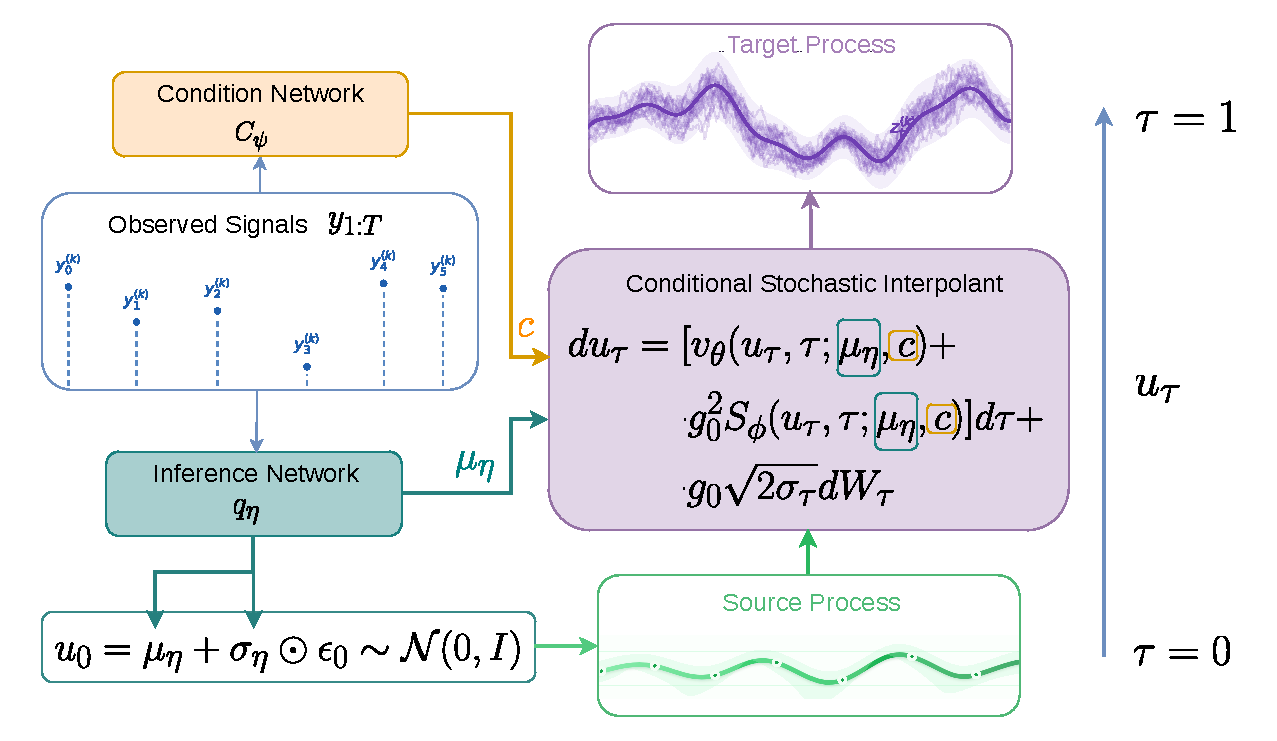
\includegraphics[width=0.9\textwidth]{figures/CondStochInterpolant.pdf}
    \caption[Computational graph of Conditional Stochastic Interpolant]{Computational graph of Conditional Stochastic Interpolant. The inference network $q_\eta$ produces the source distribution parameters $(\mu_\eta, \sigma_\eta)$ from the observations $y_{1:T}$. The conditioning network $C_\psi$ extracts conditioning information $c$ from the observations. Both the mean parameter $\mu_\eta$ and the conditioning information $c$ are taken as condition of the transport velocity network $v_\theta$ and the score network $S_\phi$, which model the deterministic and stochastic components of the interpolant dynamics, respectively. The stochastic solver integrates the interpolant SDE forward in flow time $\tau$, starting from the source trajectory $u_0$, to produce terminal trajectories that approximate samples from the posterior distribution over state trajectories.}
    \label{fig:conditional_stochastic_interpolant_graph}
\end{figure}
The learned interpolant dynamics are described by a refinement \ac{SDE} with a deterministic transport term and a score-based correction:
\begin{equation}
    du_\tau =
    \left[
        v_\theta(u_\tau, \tau; \mu_\eta, c)
        +g_0^2 S_\phi(u_\tau,\tau; \mu_\eta, c)\right]d\tau
    + g_0\sqrt{2\sigma_\tau}dW_\tau,
    \label{eq:conditional_stochastic_interpolant_general}
\end{equation}
where both neural fields, the transport velocity $v_\theta$ and the score network $S_\phi$, are conditioned on the context $c$ and on the encoder mean $\mu_\eta$. The encoder mean $\mu_\eta$ provides a state-space estimate of the trajectory and gives the SDE a physically meaningful state-space reference. Since $u_\tau$ and $v^*$ depend on the sampled source $u_0$, gradients from the flow-matching and score-matching losses propagate through the interpolant path into the inference network.

The model is trained end-to-end with a joint encoder-interpolant objective:
\begin{equation}
    \mathcal{L}_{\text{joint}}
    =
    \mathcal{L}_{\text{flow}}
    +\mathcal{L}_{\text{score}}
    +\lambda\mathcal{L}_{\text{nll}},
    \label{eq:conditional_stochastic_interpolant_loss}
\end{equation}
where
\begin{align}
    \mathcal{L}_{\text{flow}}
    &=
    \left\|
        v_\theta(u_\tau,\tau;\mu_\eta,c)-v^*
    \right\|^2, \\
    \mathcal{L}_{\text{score}}
    &=
    \left\|
        S_\phi(u_\tau,\tau;\mu_\eta,c)+\epsilon
    \right\|^2, \\
    \mathcal{L}_{\text{nll}}
    &=
    -\log
    \mathcal{N}\!\left(
        x_{1:T};
        \mu_\eta,
        \operatorname{diag}(\sigma_\eta^2)
    \right).
\end{align}
The flow loss learns the deterministic transport field, while the score loss trains the score network in a sigma-scaled form. The negative log-likelihood term trains the inference network to assign high probability to the reference state trajectory $x_{1:T}$ under the Gaussian source distribution $\mathcal{N}(\mu_\eta,\operatorname{diag}(\sigma_\eta^2))$.

For a new observation trajectory, posterior estimation is performed by evaluating the inference network once, drawing $N_p$ source particles from Equation~\ref{eq:conditional_stochastic_interpolant_source} using independent samples of $\epsilon_0$, solving Equation~\ref{eq:conditional_stochastic_interpolant_general} with an Euler--Maruyama discretization, and collecting the terminal particles $\{u_1^{(i)}\}_{i=1}^{N_p}$. These terminal trajectories represent samples from the approximate posterior $p(x_{1:T}| y_{1:T})$.

CondStochInterpolant therefore acts as a refinement filter. It does not require a separate generative decoder for the source distribution; instead, the stochastic inference network produces an adaptive initial particle distribution, and the refinement \ac{SDE} transports those particles into a calibrated and potentially multimodal posterior over full state trajectories.

\subsubsection{Numerical Results}
\begin{figure}[ht]
    \centering
    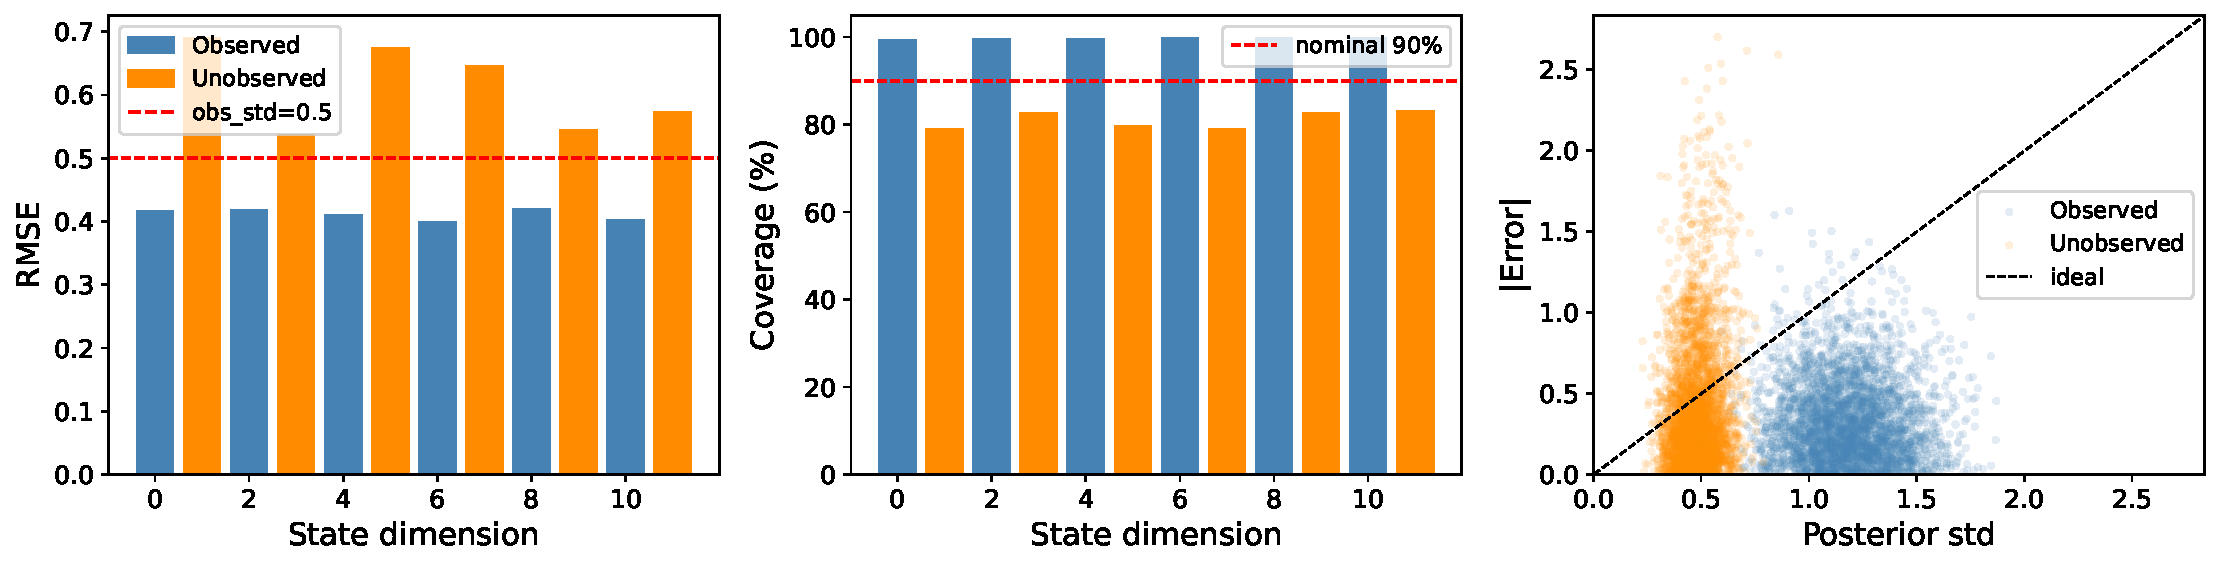
\includegraphics[width=\textwidth]{figures/SI_segev100_diagnostics.pdf}
    \caption[Performance of CondStochInterpolant]{Estimation Accuracy and Calibration Diagnostics of CondStochInterpolant. The left panel shows the \ac{RMSE} of the posterior mean trajectory against the reference state trajectory. The center panel shows the confidence interval coverage probability of the posterior predictive distribution. The nominal coverage probability is 90\%. In the right panel, the calibration scatter plot compares posterior standard deviations with realized absolute estimation errors.}
    \label{fig:si_diagnostics}
\end{figure}

\begin{figure}[ht]
    \centering
    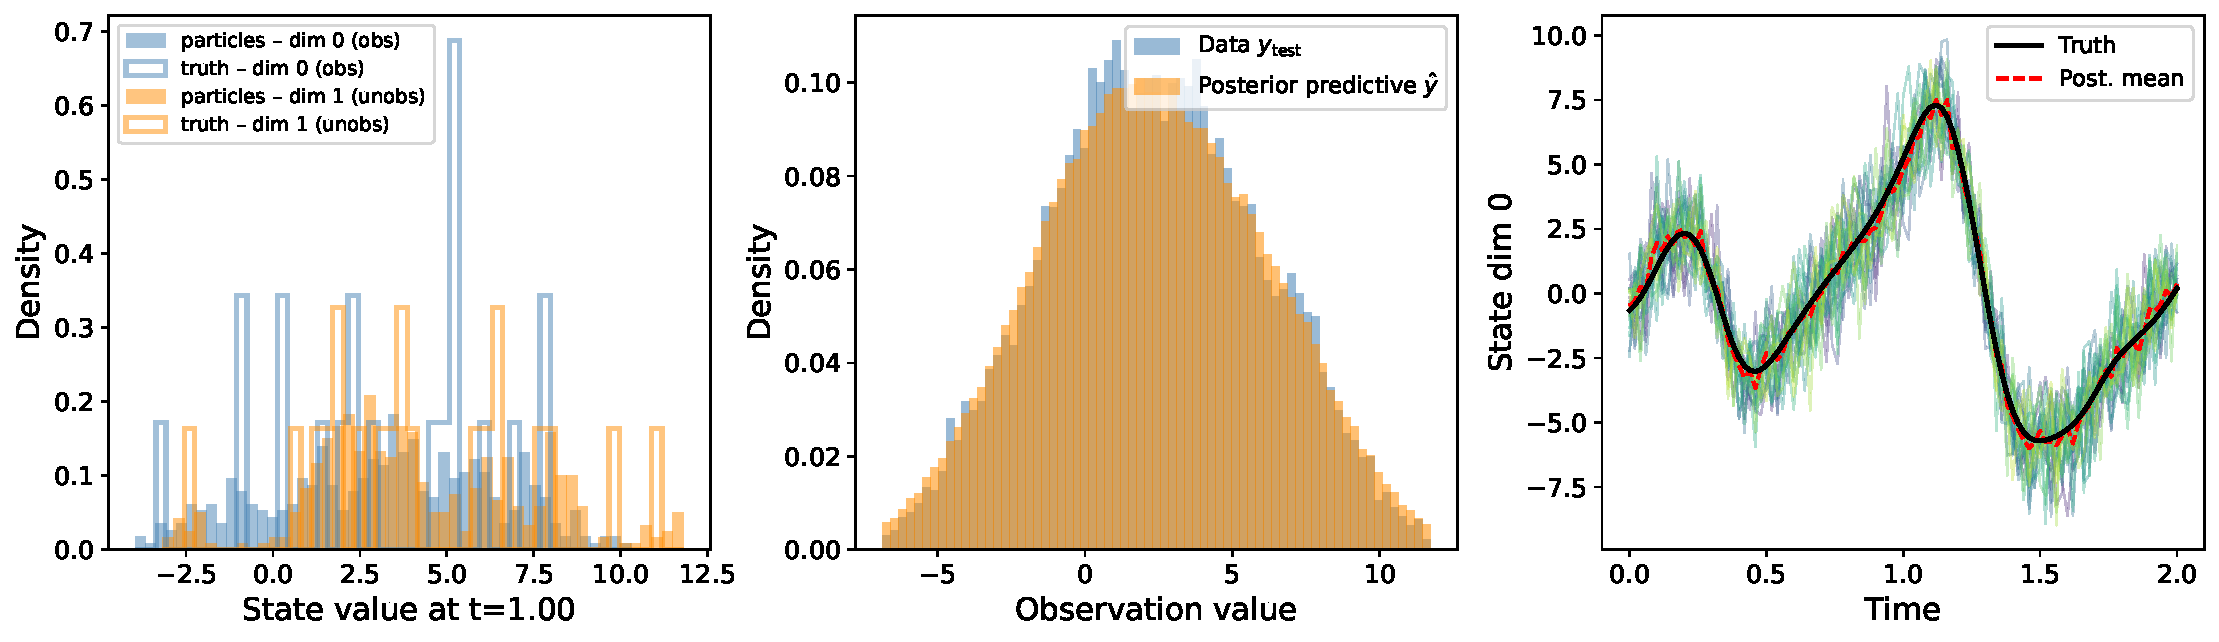
\includegraphics[width=\textwidth]{figures/SI_segev100_multimodal.pdf}
    \caption[Multi-modality of CondStochInterpolant]{Posterior Multi-modality and Predictive Consistency of CondStochInterpolant. The left panel compares the particle distribution against the ground-truth state values. The center panel compares the empirical distribution of the test observations with the posterior predictive distribution. The right panel shows posterior particle trajectories for a representative state dimension.}
    \label{fig:si_multimodal}
\end{figure}

\begin{figure}[ht]
    \centering
    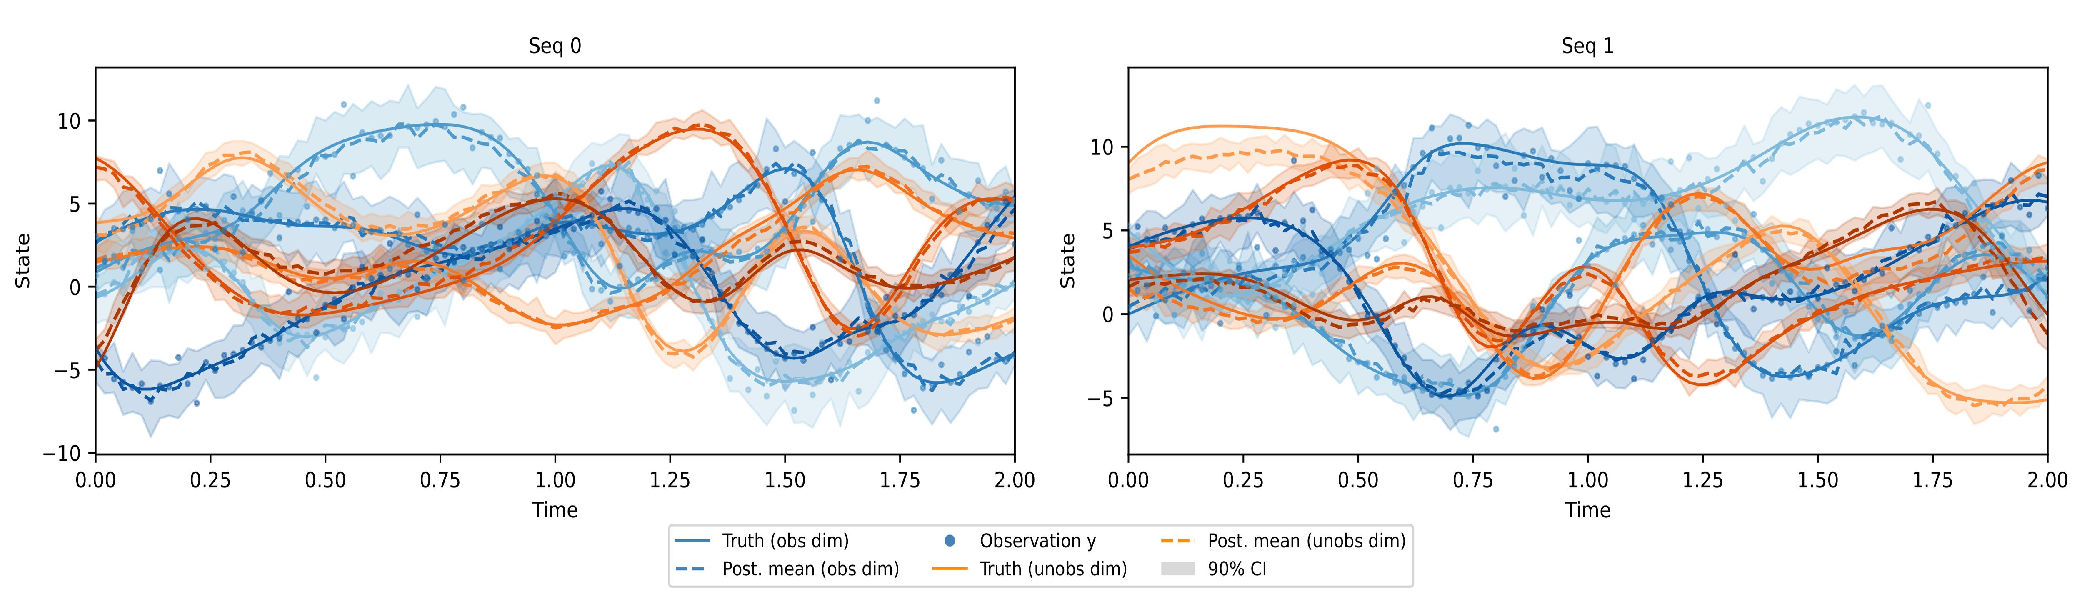
\includegraphics[width=\textwidth]{figures/SI_segev100_trajectories.pdf}
    \caption[Trajectory Reconstruction of CondStochInterpolant]{Trajectory Reconstruction and Uncertainty Quantification of CondStochInterpolant. Two representative test sequences are illustrated, where the curves are the posterior mean and the bands are 90\% confidence intervals.   The blue dots are the observed data points. The blue curves represent the observed trajectories while the red curves show the predicted trajectories.}
    \label{fig:si_trajectories}
\end{figure}

The observation noise is the same as that in the FlowSDE experiments. The full-horizon results are shown in Figures~\ref{fig:si_diagnostics}, \ref{fig:si_multimodal}, and \ref{fig:si_trajectories}.

Figure~\ref{fig:si_diagnostics} summarizes the estimation accuracy and calibration behavior. The posterior mean reconstructs observed coordinates more accurately than unobserved coordinates, as expected from the partial-observation setting. The \ac{RMSE} is approximately $0.4$ on observed states and approximately $0.6$ on unobserved states, which is close to the observation-noise scale of $0.5$. This indicates that the refinement process successfully transfers information from observed coordinates to hidden ones, but the unobserved components remain intrinsically harder because they must be inferred through the learned dynamics and cross-coordinate correlations. The empirical coverage is close to the nominal $90\%$ level, suggesting that the posterior bands are not merely narrow point-estimation intervals but carry meaningful uncertainty. The calibration scatter further supports this interpretation: larger posterior standard deviations tend to coincide with larger realized errors, so the model assigns higher uncertainty to cases where its estimates are less reliable.

Figure~\ref{fig:si_multimodal} illustrates the distributional behavior of the posterior particles. The particle distribution is concentrated around the reference state values while retaining a visible spread, which shows that CondStochInterpolant does not collapse to a single deterministic trajectory. The comparison between the empirical observation distribution and the posterior predictive distribution suggests that the model captures the broad shape of the noisy data distribution, including the heavy-tailed and multimodal effects introduced by the mixture noise. The representative particle trajectories also show that uncertainty is propagated coherently through time rather than appearing as independent pointwise noise. This is important for state estimation, since plausible posterior samples should remain dynamically consistent over the full horizon.

The trajectory reconstructions in Figure~\ref{fig:si_trajectories} provide a more local view of this behavior. For the displayed test sequences, the posterior mean follows the reference trajectory closely over most of the horizon, while the $90\%$ confidence bands widen around more uncertain or rapidly changing regions. The observed data points are noisy and occasionally deviate from the underlying state, but the inferred trajectories remain smoother than the raw observations. This indicates that the model uses the refinement \ac{SDE} as a denoising and state-completion mechanism rather than directly interpolating noisy measurements. 

Overall, the results show that CondStochInterpolant achieves a favorable balance between reconstruction accuracy, uncertainty calibration, and posterior diversity under multimodal observation noise.